%  LaTeX support: latex@mdpi.com 
%  For support, please attach all files needed for compiling as well as the log file, and specify your operating system, LaTeX version, and LaTeX editor.

%=================================================================
\documentclass[pharmaceuticals,article,submit,pdftex,moreauthors]{Definitions/mdpi} 

%=================================================================
% MDPI internal commands - do not modify
\firstpage{1} 
\makeatletter 
\setcounter{page}{\@firstpage} 
\makeatother
\pubvolume{1}
\issuenum{1}
\articlenumber{0}
\pubyear{2026}
\copyrightyear{2026}
\datereceived{ } 
\daterevised{ } % Comment out if no revised date
\dateaccepted{ } 
\datepublished{ } 

%=================================================================
% Add packages and commands here. 
\graphicspath{ {images/} }

%=================================================================
% Full title of the paper (Capitalized)
\Title{Targeting Diverse Human Coronaviruses with a Single Small Molecule: Computational Assessment of CKP-25 as a Promising Broad-Spectrum Receptor-Binding Anchor}

% % Author Orchid ID: enter ID or remove command
% \newcommand{\orcidauthorA}{0000-0000-0000-0000} % Add \orcidA{} behind the author's name

% % Authors, for the paper (add full first names)
% \Author{Anonymous $^{1,*}$\orcidA{}}

% % MDPI internal command: Authors, for metadata in PDF
% \AuthorNames{Anonymous}

% % Affiliations / Addresses
% \address{%
% $^{1}$ \quad University of Nowhere; anonymous@unowhere.edu}

% % Contact information of the corresponding author
% \corres{Correspondence: anonymous@unowhere.edu}

% Author ORCID IDs
\newcommand{\orcidauthorA}{0009-0000-8117-312X}
\newcommand{\orcidauthorB}{0000-0001-9094-3480}
\newcommand{\orcidauthorC}{0000-0001-7400-9591}
\newcommand{\orcidauthorD}{0000-0003-3814-6710}

% Authors
\Author{
Angelos-Michael Papadopoulos $^{1,2,*}$\orcidA{},
Spyros Petrakis $^{3,*}$\orcidB{},
Federico Alvarez $^{2}$\orcidC{}
and Petros Daras $^{1}$\orcidD{}
}

% Authors for PDF metadata
\AuthorNames{
Angelos-Michael Papadopoulos,
Spyros Petrakis,
Federico Alvarez
and Petros Daras
}

% Affiliations / Addresses
\address{%
$^{1}$ \quad Information Technologies Institute, Centre for Research and
Technology Hellas (CERTH), 6th km Charilaou--Thermi Road,
57001 Thermi, Thessaloniki, Greece;\\
$^{2}$ \quad Universidad Polit\'ecnica de Madrid,
28040 Madrid, Spain;\\
$^{3}$ \quad Institute of Applied Biosciences, Centre for Research and
Technology Hellas (CERTH), 6th km Charilaou--Thermi Road,
57001 Thermi, Thessaloniki, Greece
}

% Corresponding authors
\corres{
Correspondence: angepapa@iti.gr;
spetrak@certh.gr
}




\abstract{
\textbf{Background/Objectives:}
The emergence of novel coronaviruses highlights the critical need for broad-spectrum antiviral strategies targeting conserved mechanisms of viral entry. CKP-25 was recently reported as a small-molecule inhibitor of the SARS-CoV-2 spike receptor-binding domain. This study aimed to assess computationally whether CKP-25 can maintain stable binding at receptor-recognition interfaces across phylogenetically diverse human coronaviruses.
\textbf{Methods:}
CKP-25 was docked to the spike receptor-binding regions of Middle East respiratory syndrome coronavirus (MERS-CoV), severe acute respiratory syndrome coronavirus 1 (SARS-CoV-1), and human coronaviruses NL63, 229E, and HKU1 (HCoV-NL63, HCoV-229E, and HCoV-HKU1). Each selected complex was subjected to a 100 ns all-atom molecular dynamics (MD) simulation. Binding stability was evaluated using protein and ligand root-mean-square deviation (RMSD), residue flexibility, radius of gyration, protein--ligand contact persistence, polar interactions, and Molecular Mechanics--Generalized Born Surface Area (MM-GBSA) calculations.
\textbf{Results:}
CKP-25 remained at the targeted interfaces in all five systems and generally exhibited low ligand RMSD plateaus, mostly below 2.0~\AA. Contact analyses indicated a shared dependence on shape-complementary van der Waals packing involving hydrophobic and aromatic residues, including tyrosine- and tryptophan-rich anchoring environments. MM-GBSA estimates ranged from $-22.84$ to $-37.47$ kcal/mol and supported two relative binding-energy tiers, with MERS-CoV and HCoV-NL63 showing the most favorable values, followed by SARS-CoV-1, HCoV-HKU1, and HCoV-229E. This ranking was broadly consistent with the structural-stability and contact-frequency analyses.
\textbf{Conclusions:}
These results support CKP-25 as a potential broad-spectrum receptor-interface binding scaffold for human coronaviruses. Experimental binding and viral-entry inhibition studies are required to validate the predicted cross-coronavirus binding behavior.
}

% Keywords

\keyword{broad-spectrum antiviral; coronavirus; CKP-25; molecular docking; molecular dynamics; receptor-binding interface; MM-GBSA}


%=================================================================
\begin{document}



\section{Introduction}
The recurrent emergence of highly pathogenic human coronaviruses (HCoVs) over the past two decades, most notably Severe Acute Respiratory Syndrome Coronavirus (SARS-CoV-1), Middle East Respiratory Syndrome Coronavirus (MERS-CoV), and SARS-CoV-2, has underscored the pandemic potential of this viral family \cite{cui2019origin, hu2021characteristics}. Alongside these highly virulent strains, endemic coronaviruses such as HCoV-NL63, HCoV-229E, and HCoV-HKU1 persistently circulate within the human population, contributing significantly to seasonal respiratory diseases \cite{su2016epidemiology, wilson2024global}. The continuous evolution and cross-species transmission of coronaviruses emphasize the urgent need for broad-spectrum antiviral therapeutics capable of targeting conserved mechanisms of viral infection.

Viral entry into the host cell is a critical bottleneck in the coronavirus life cycle and represents a primary target for drug discovery \cite{bosch2003severe}. This process is mediated by the viral Spike (S) glycoprotein, a massive homotrimeric fusion protein. While the specific host receptors vary among strains, for instance, SARS-CoV-1 and HCoV-NL63 utilize Angiotensin-Converting Enzyme 2 (ACE2), MERS-CoV binds Dipeptidyl Peptidase 4 (DPP4), and HCoV-229E relies on Aminopeptidase N (APN), the structural mechanism of receptor engagement is highly conserved \cite{li2016structure, walls2020structure, mahdi2025receptor}. Consequently, small molecules that can act as broad-spectrum anchors at the receptor-binding interfaces of diverse spike proteins offer a promising strategy to neutralize viral entry and mitigate the risk of viral escape mutations \cite{prajapat2020drug, lyles2025entry}.

In this study, we evaluate the therapeutic potential of CKP-25, a small-molecule inhibitor of SARS-CoV-2, as a candidate broad-spectrum viral entry inhibitor against HCoVs, building on its previously reported activity \cite{gkekas2024ai}. CKP-25 was previously shown to protect human cells from SARS-CoV-2 infection, significantly suppressing viral titers \textit{in vitro}. Its therapeutic effect is attributed to its stable binding on the interface between the SARS-CoV-2 spike Receptor-Binding Domain (RBD) and its ACE2 receptor, which is widely expressed on the cell surface of the human respiratory system \cite{zhao2020virus}. We hypothesized that CKP-25 would remain associated with receptor-recognition interfaces across phylogenetically diverse human coronaviruses by exploiting shared hydrophobic and aromatic physicochemical features, despite differences in sequence and host-receptor usage.

To assess the binding potential and structural stability of CKP-25, we employed an integrative computational pipeline combining molecular docking with extensive molecular dynamics (MD) simulations. While static docking provides initial binding poses, the highly dynamic nature of the spike protein, which undergoes large-scale conformational transitions between open (receptor-accessible) and closed (receptor-inaccessible) states of its receptor-binding domains (RBDs) \cite{walls2020structure, lu2020real}, necessitates advanced physics-based simulations to validate the dynamic stability under the simulated conditions of the ligand-receptor complex \cite{hollingsworth2018molecular}. Therefore, we subjected the CKP-25/spike complexes of five phylogenetically diverse coronaviruses (MERS-CoV, SARS-CoV-1, HCoV-NL63, HCoV-229E, and HCoV-HKU1) to 100-ns all-atom MD simulations. By analyzing geometric stability metrics, tracking protein--ligand contact persistence, and calculating relative binding free-energy estimates via the Molecular Mechanics-Generalized Born Surface Area (MM-GBSA) method, we provide a comparative computational assessment of CKP-25 as a broad-spectrum spike protein inhibitor. The overall computational workflow is summarized in Figure \ref{fig:workflow}.


\begin{figure}[H]
\centering

\includegraphics[width=\textwidth]{images/workflow.pdf}
\caption{\textbf{Computational workflow for evaluating CKP-25 binding across diverse human coronavirus spike interfaces.} Experimentally determined spike receptor-binding structures from five human coronaviruses (PDB IDs: 8Y7Y, 3KBH, 4KR0, 6ATK, and 2AJF) were retrieved, and residues located within 4.0~\AA{} of the corresponding host receptor or entry mediator were used to define target-specific receptor-interface docking regions. GNINA-guided molecular docking was then used to generate initial CKP-25 binding poses for five 100-ns explicit-solvent molecular dynamics (MD) simulations. Structural stability metrics, including root-mean-square deviation (RMSD), root-mean-square fluctuation (RMSF), radius of gyration ($R_g$), and protein--ligand contact persistence, were evaluated over the complete production trajectories. Molecular Mechanics--Generalized Born Surface Area (MM-GBSA) calculations were performed using the equilibrated 50--100~ns window. The comparative analysis supported two relative predicted binding-energy tiers, with MERS-CoV and HCoV-NL63 forming the more favorable tier, followed by SARS-CoV-1, HCoV-HKU1, and HCoV-229E.}
\label{fig:workflow}
\end{figure}



\section{Results}
% \subsection{HCoV spike target selection}
% To evaluate the potential broad-spectrum receptor-interface binding of CKP-25, an initial virtual structural assessment was performed using established experimental models of coronavirus entry. High-resolution three-dimensional structures of spike (S) glycoprotein receptor-binding regions from alpha- and betacoronaviruses---specifically HCoV-NL63, HCoV-229E, MERS-CoV, SARS-CoV-1, and HCoV-HKU1---in complex with their respective host-cell receptors or entry mediators were selected. These included:
% \begin{itemize}
%     \item \textbf{MERS-CoV B-spike}: Crystallographic structure of the receptor-binding domain complexed with human dipeptidyl peptidase 4 (DPP4) receptor at 2.70 \AA\ resolution (PDB: 4KR0) \cite{lu2013molecular}.
%     \item \textbf{SARS-CoV-1 E-spike}: Crystallographic structure of the receptor-binding domain complexed with human ACE2 receptor at 2.90 \AA\ resolution (PDB: 2AJF) \cite{li2005structure}.
%     \item \textbf{HCoV-NL63 E-spike}: Crystallographic structure of the receptor-binding domain complexed with human ACE2 receptor at 3.31 \AA\ resolution (PDB: 3KBH) \cite{wu2009structure}.
%     \item \textbf{HCoV-229E E-spike}: Crystallographic structure of the receptor-binding domain complexed with human aminopeptidase N (APN) receptor at 3.50 \AA\ resolution (PDB: 6ATK) \cite{wong2017crystal}.
%     \item \textbf{HCoV-HKU1 A-spike}: Cryo-electron microscopy structure of the spike protein receptor-binding domain complexed with human transmembrane serine protease 2 (TMPRSS2) receptor at 3.24 \AA\ resolution (PDB: 8Y7Y) \cite{wang2024tmprss2}.
% \end{itemize}

% These structures served as templates for comparative molecular docking simulations, aiming to assess whether CKP-25 can stably occupy receptor-binding interfaces across highly divergent human coronaviruses, similar to its reported inhibitory effect on the SARS-CoV-2 S-RBD/ACE2 interaction.

\subsection{Selected Human Coronavirus Spike Targets}

Application of the structural selection criteria described in
Section ~\ref{sec:target_selection} yielded a panel of five experimentally
resolved human coronavirus spike--host complexes: MERS-CoV (4KR0),
SARS-CoV-1 (2AJF), HCoV-NL63 (3KBH), HCoV-229E (6ATK), and HCoV-HKU1
(8Y7Y). The panel included both alpha- and betacoronaviruses and
represented distinct host-receptor or entry-mediator usage, including
ACE2, DPP4, APN, and TMPRSS2.

Native interface mapping identified a spatially defined
receptor-recognition hotspot for each spike target. These target-specific
hotspots were retained after removal of the host-partner coordinates and
were used to direct focused docking of CKP-25. Thus, the final panel
enabled comparative evaluation of CKP-25 at structurally and
phylogenetically diverse coronavirus receptor-recognition interfaces.



\subsection{Molecular Docking Affinities}
Static molecular docking was performed to generate the initial binding poses of CKP-25 for the subsequent MD simulations. The GNINA-reported docking affinities indicated generally favorable interactions for CKP-25 across all targets (see Table \ref{affinity_scores}).

\begin{table}[H]
\caption{GNINA Docking Affinities for CKP-25.\label{affinity_scores}}
\centering
\begin{tabular}{lc}
\toprule
\textbf{System (PDB)} & \textbf{Docking Affinity (kcal/mol)} \\
\midrule
HCoV-HKU1 A-spike (8Y7Y)  & -6.76 \\
MERS-CoV B-spike (4KR0)   & -6.61 \\
HCoV-NL63 E-spike (3KBH)  & -6.32 \\
SARS-CoV-1 E-spike (2AJF) & -6.18 \\
HCoV-229E E-spike (6ATK)  & -5.93 \\
\bottomrule
\end{tabular}
\end{table}

While all static docking affinity scores were encouraging ($<-5.9$ kcal/mol), it is crucial to note that they did not perfectly predict the final thermodynamic hierarchy observed in the dynamic MM-GBSA calculations (Section ~\ref{sec:MM-GBSA}). For instance, HCoV-HKU1 achieved the best static docking affinity but demonstrated only moderate predicted binding after MD/MM-GBSA evaluation, whereas MERS-CoV and HCoV-NL63 exhibited more favorable predicted binding under dynamic simulation. This discrepancy highlights the importance of using 100-ns MD simulations to evaluate static docking poses, as the dynamic plasticity of the spike protein can significantly influence ligand stability and comparative binding rankings. Notably, this difference is not driven by major structural displacement of the ligand, as both MERS-CoV and HCoV-HKU1 show highly stable ligand RMSD plateaus ($\leq 1.3$~\AA{} relative to the starting pose; see Section ~\ref{rec:Equilibration} ). Instead, the discrepancy is thermodynamic in nature: the HCoV-HKU1 interface offers fewer complementary hydrophobic packing partners ($\Delta E_{\text{vdw}} = -29.01$ kcal/mol) compared to the highly optimized aromatic pocket of MERS-CoV ($\Delta E_{\text{vdw}} = -41.90$ kcal/mol), yielding weaker overall binding free energy despite equivalent initial pose stability. The starting docked configurations, demonstrating the shape-complementary insertion of CKP-25 into the receptor-binding interfaces, are illustrated in Figure \ref{fig:docked_poses_5panel}.

\begin{figure}[H]
\centering
\includegraphics[width=\textwidth]{images/5_covid_targets_best_pose_with_cpk25.pdf}
\caption{\textbf{Starting molecular docking configurations of CKP-25 bound to the host-receptor interfaces of five target human coronavirus spike proteins.} Panels show: (A) MERS-CoV (PDB 4KR0), (B) HCoV-NL63 (PDB 3KBH), (C) SARS-CoV-1 (PDB 2AJF), (D) HCoV-HKU1 (PDB 8Y7Y), and (E) HCoV-229E (PDB 6ATK). Each panel displays the full complex on the left with a zoomed-in inset on the right highlighting atomic-level contacts for key interface residues.}
\label{fig:docked_poses_5panel}
\end{figure}

\subsection{System Equilibration and CKP-25 Binding Stability}
\label{rec:Equilibration}
The structural stability of each protein--ligand complex was monitored via the C$\alpha$ RMSD of the protein backbone throughout the 100-ns trajectory (Figure \ref{fig:md_protein_rmsd}). All five systems followed a consistent pattern: an initial increase in C$\alpha$ RMSD during approximately the first 10--20 ns, reflecting relaxation from the position-restrained equilibration state, followed by convergence to a stable plateau for the remainder of the simulation. 

Importantly, persistent binding of CKP-25 at the receptor-binding interface was observed across all five coronavirus spike proteins. Ligand RMSD, computed relative to the top-scored docked pose after C$\alpha$-based fitting, stabilized rapidly and remained mostly below 2.0 Å, converging to low-RMSD plateaus throughout the production simulations (Figure \ref{fig:md_ligand_rmsd} and Figure \ref{fig:md_ligand_boxplot}, summarized in Table \ref{tab:md_stability}). The tightest retention was observed in the HCoV-NL63 E-spike complex ($\sim 0.8$ \AA\ plateau) and SARS-CoV-1 E-spike complex ($\sim 0.9$ \AA\ plateau).

\begin{table}[htbp]
\caption{MD stability summary for all five CKP-25 coronavirus spike complexes.\label{tab:md_stability}}
\centering
\begin{tabular}{lcc}
\toprule
\textbf{System (PDB)} & \textbf{Protein C$\alpha$ RMSD} & \textbf{Ligand RMSD} \\
 & \textbf{Plateau (\AA)} & \textbf{Plateau (\AA)} \\
\midrule
MERS-CoV B-spike (4KR0)   & $\sim 1.4$ & $\sim 1.1$ \\
SARS-CoV-1 E-spike (2AJF) & $\sim 3.2$ & $\sim 0.9$ \\
HCoV-229E E-spike (6ATK)  & $\sim 1.5$ & $\sim 1.3$ \\
HCoV-HKU1 A-spike (8Y7Y)  & $\sim 1.7$ & $\sim 1.3$ \\
HCoV-NL63 E-spike (3KBH)  & $\sim 3.3$ & $\sim$ \textbf{0.8} \\
\bottomrule
\end{tabular}
\end{table}

\begin{figure}[htbp]
\centering
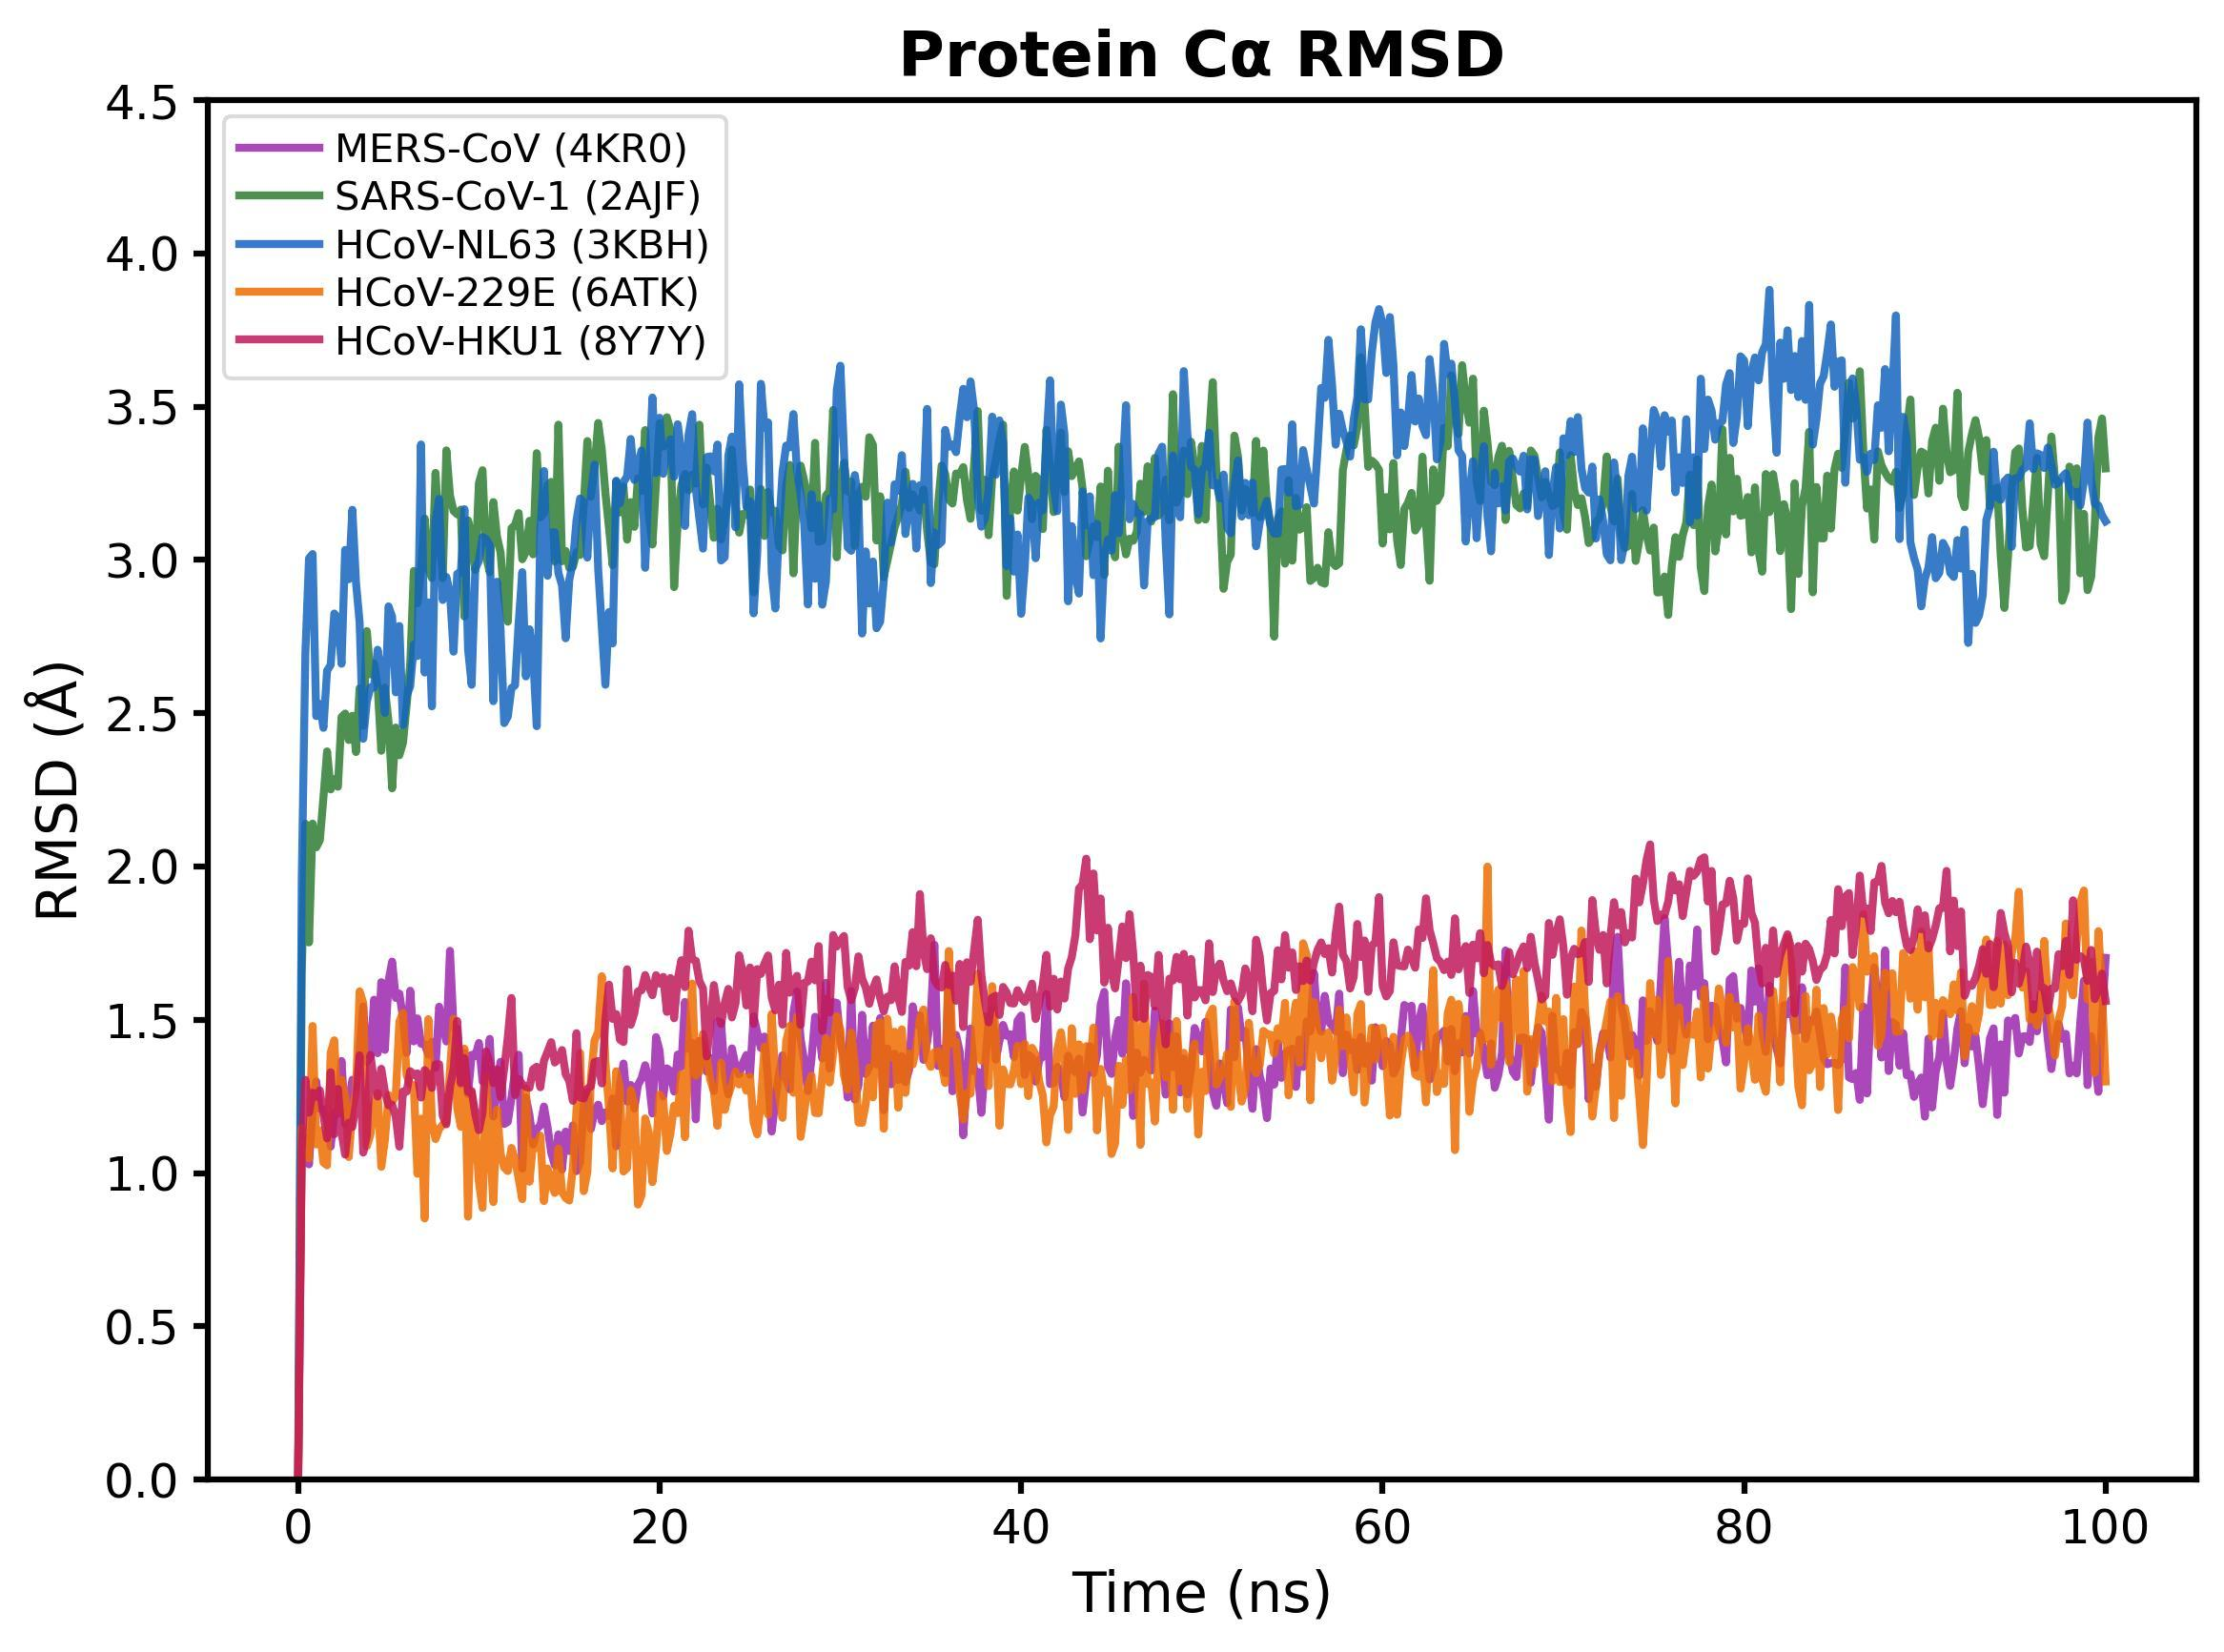
\includegraphics[width=0.75\textwidth]{images/md_protein_rmsd.jpg}
\caption{Protein backbone C$\alpha$ root-mean-square deviation (RMSD) profiles for the five CKP-25 coronavirus spike complexes over 100-ns production simulations. All systems show stable convergence within the first 10--20 ns of trajectory.}
\label{fig:md_protein_rmsd}
\end{figure}

\begin{figure}[htbp]
\centering
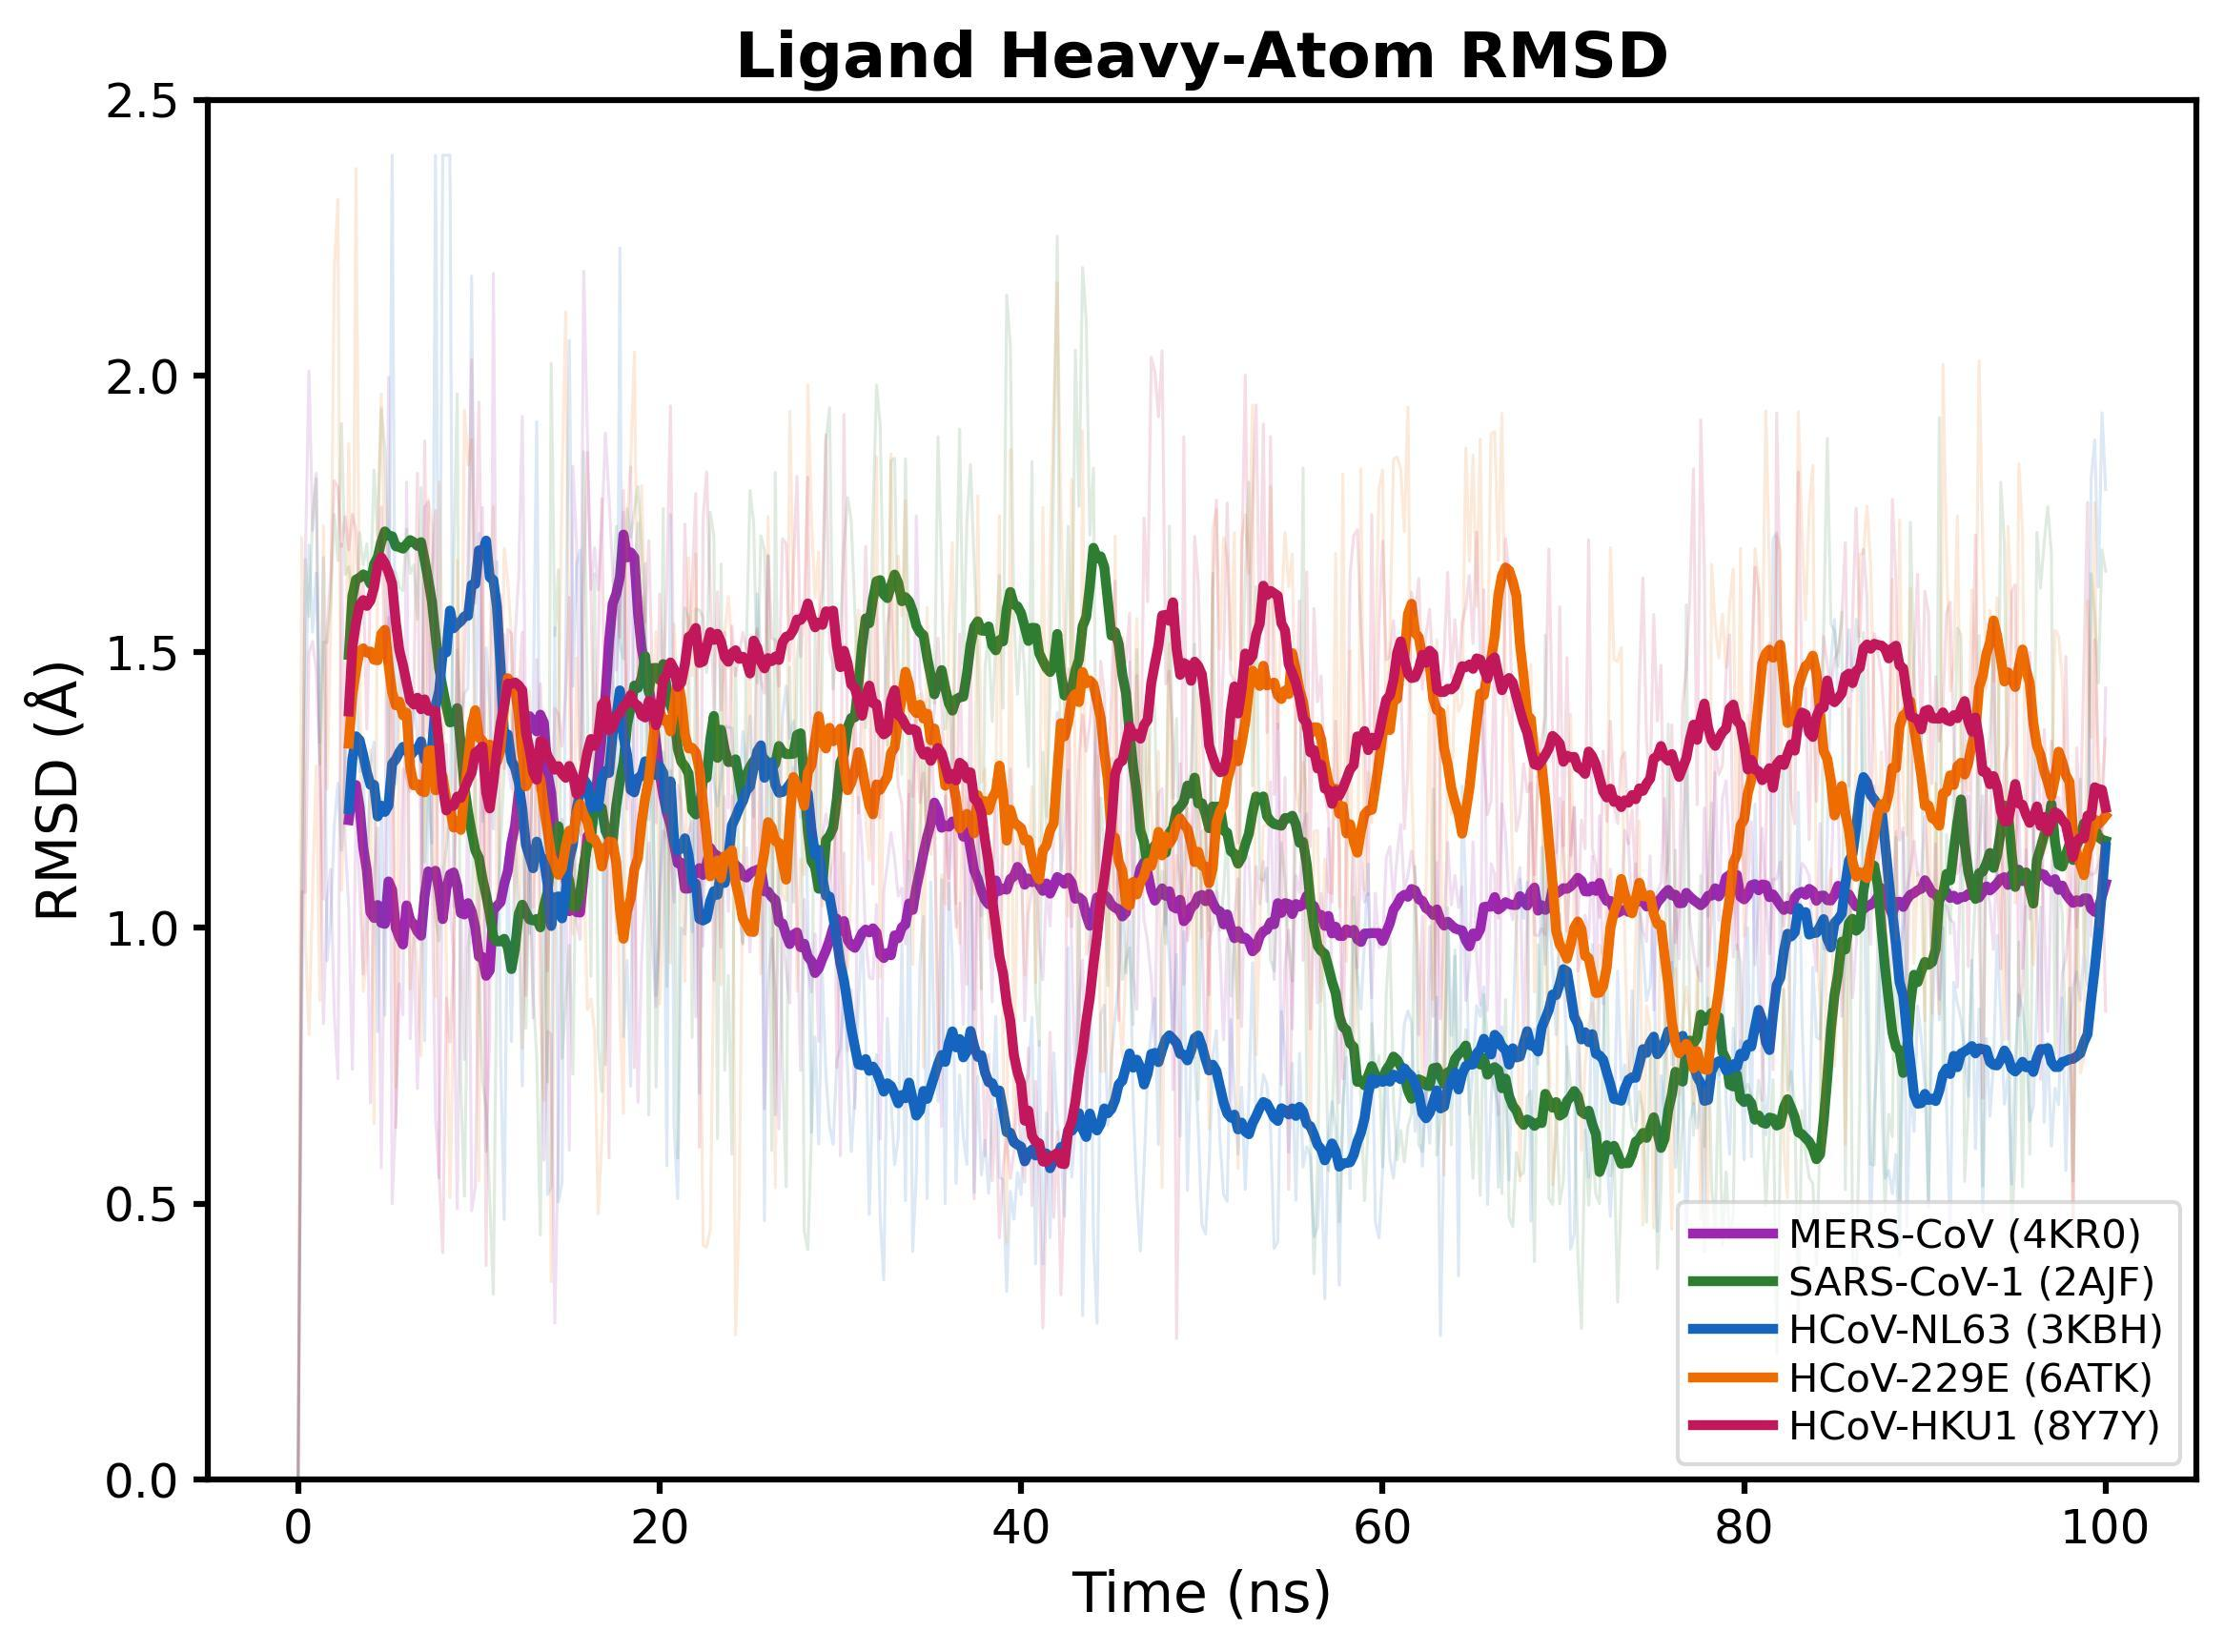
\includegraphics[width=0.75\textwidth]{images/md_ligand_rmsd.jpg}
\caption{Ligand heavy-atom RMSD profiles of CKP-25 bound to the five coronavirus spike RBDs over 100 ns. Faint lines represent raw high-frequency data, while solid lines show the moving average (15-frame window), highlighting stable low-RMSD plateaus.}
\label{fig:md_ligand_rmsd}
\end{figure}

\begin{figure}[htbp]
\centering
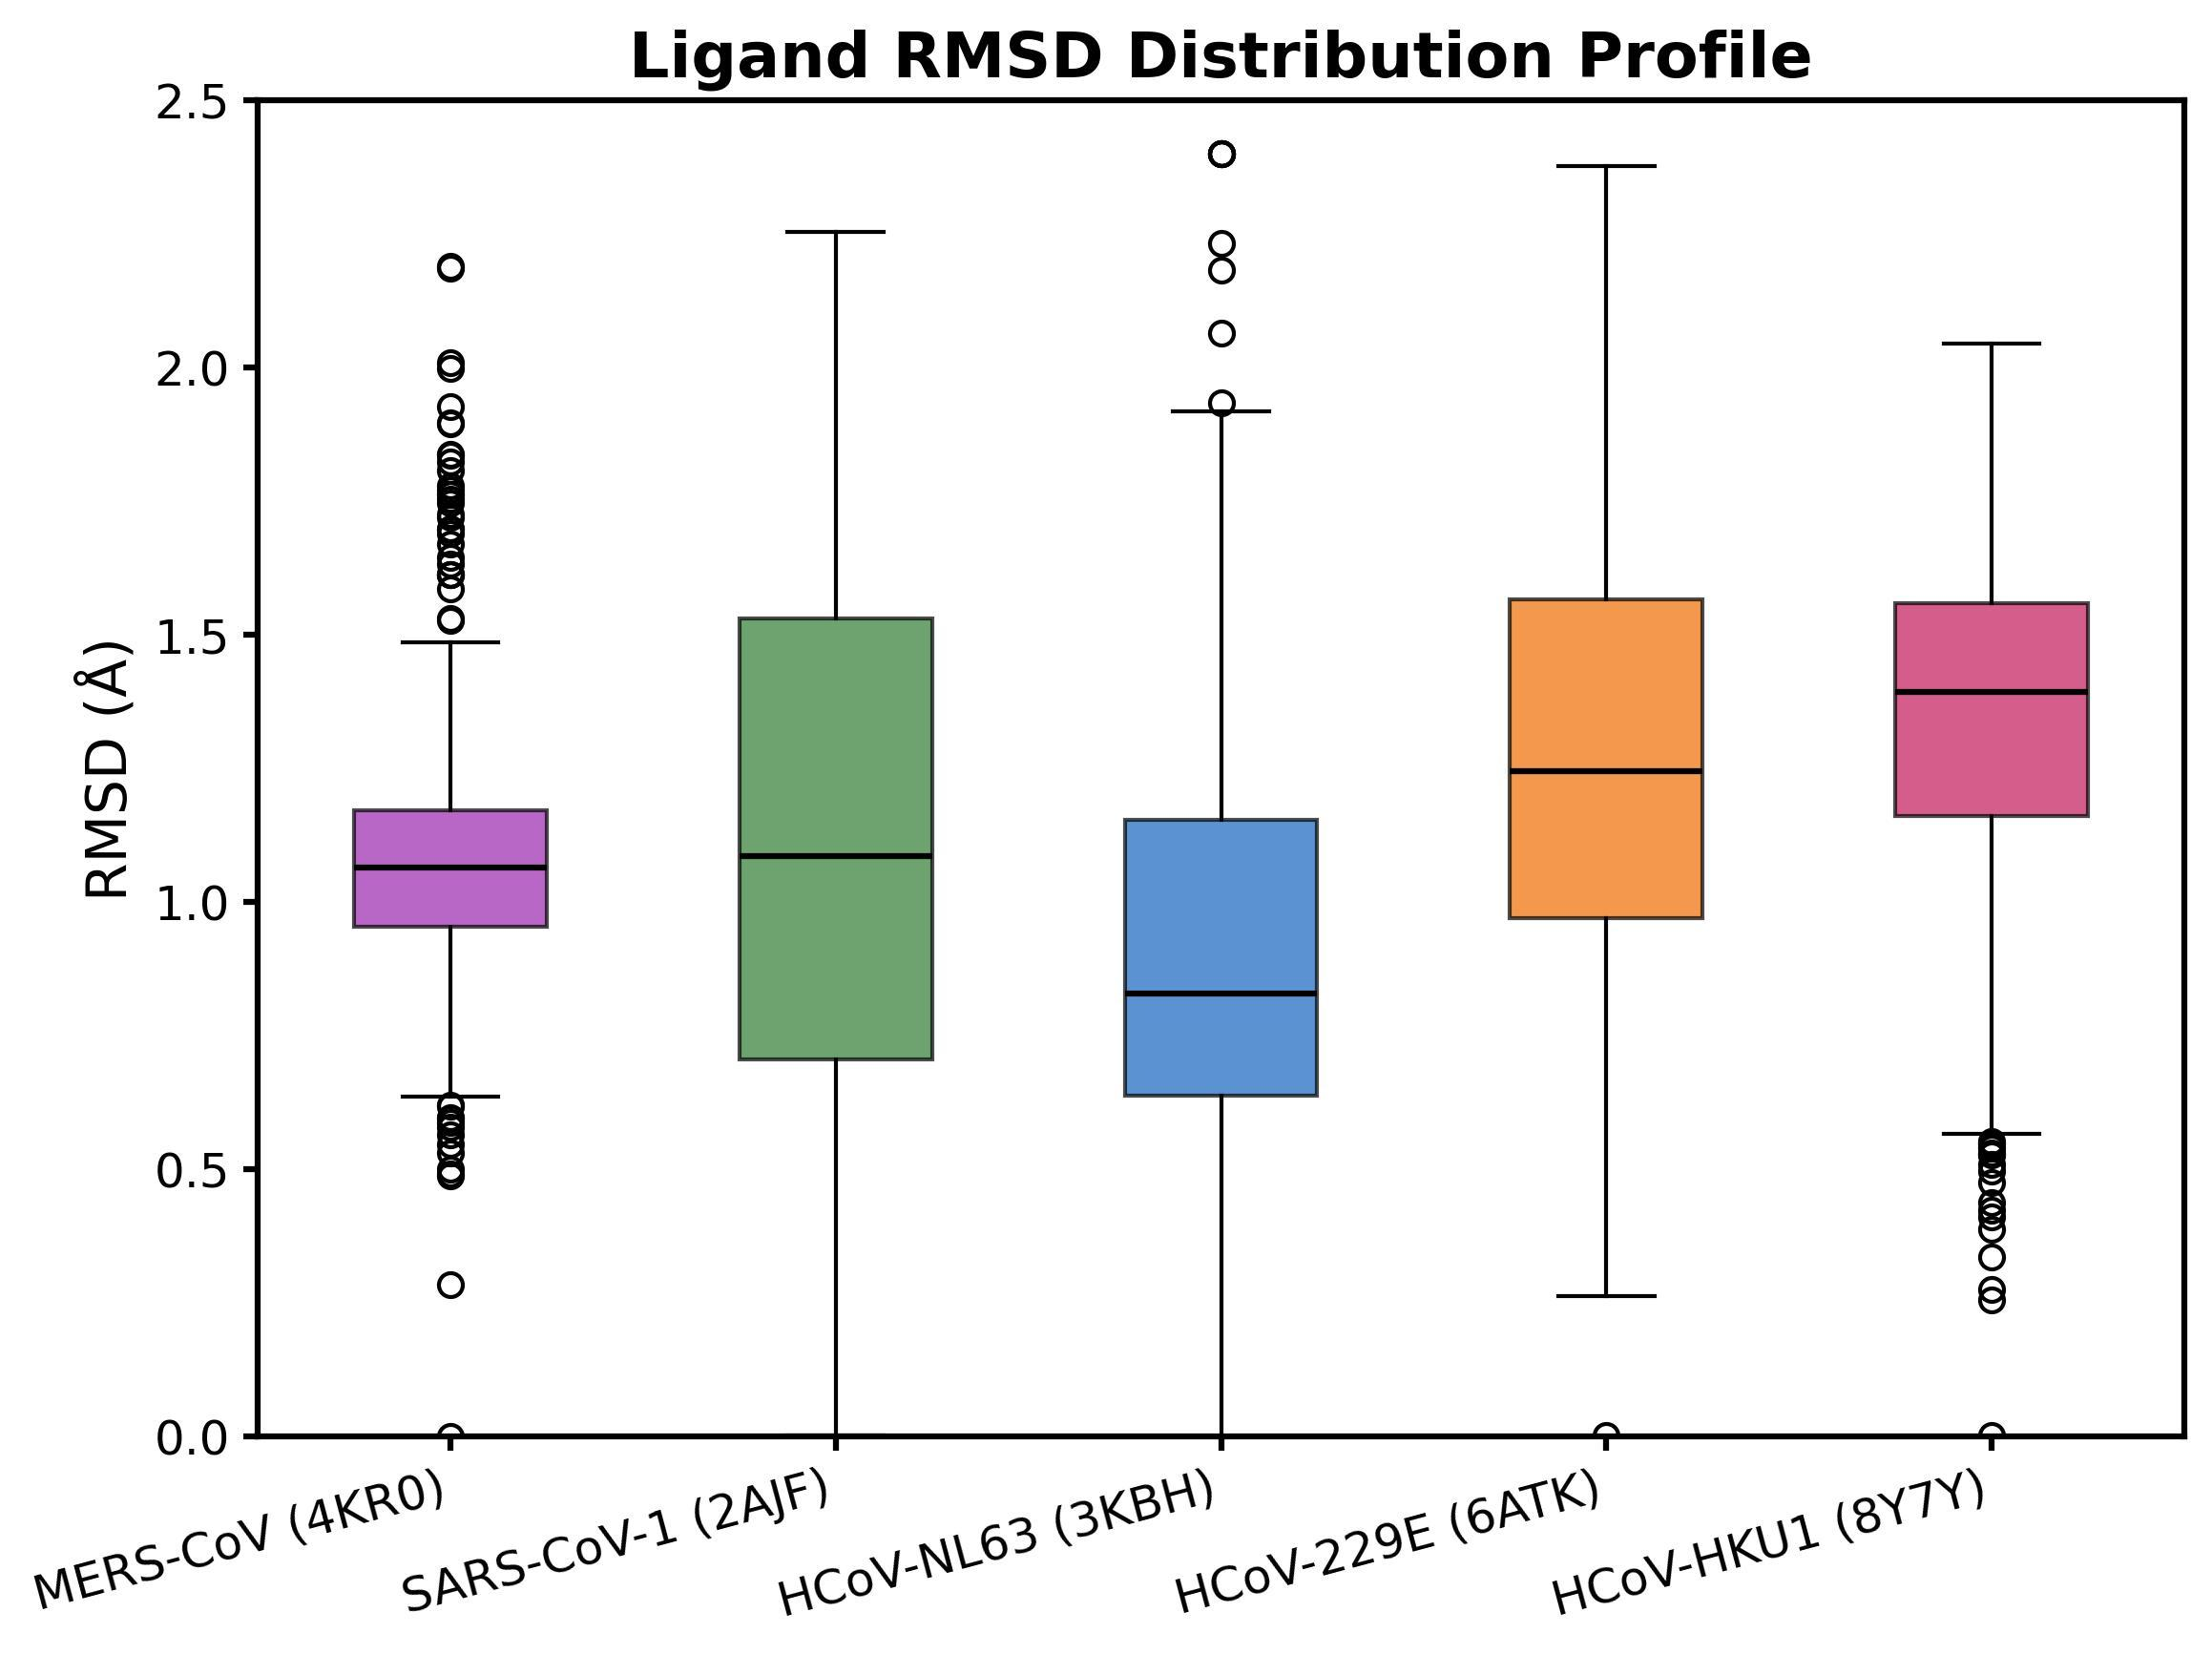
\includegraphics[width=0.75\textwidth]{images/md_ligand_boxplot.jpg}
\caption{Boxplot profile comparing the distribution and variance of ligand RMSD values across the five target complexes over the production trajectories, demonstrating generally low positional fluctuation with limited transient excursions.}
\label{fig:md_ligand_boxplot}
\end{figure}

\begin{figure}[htbp]
\centering
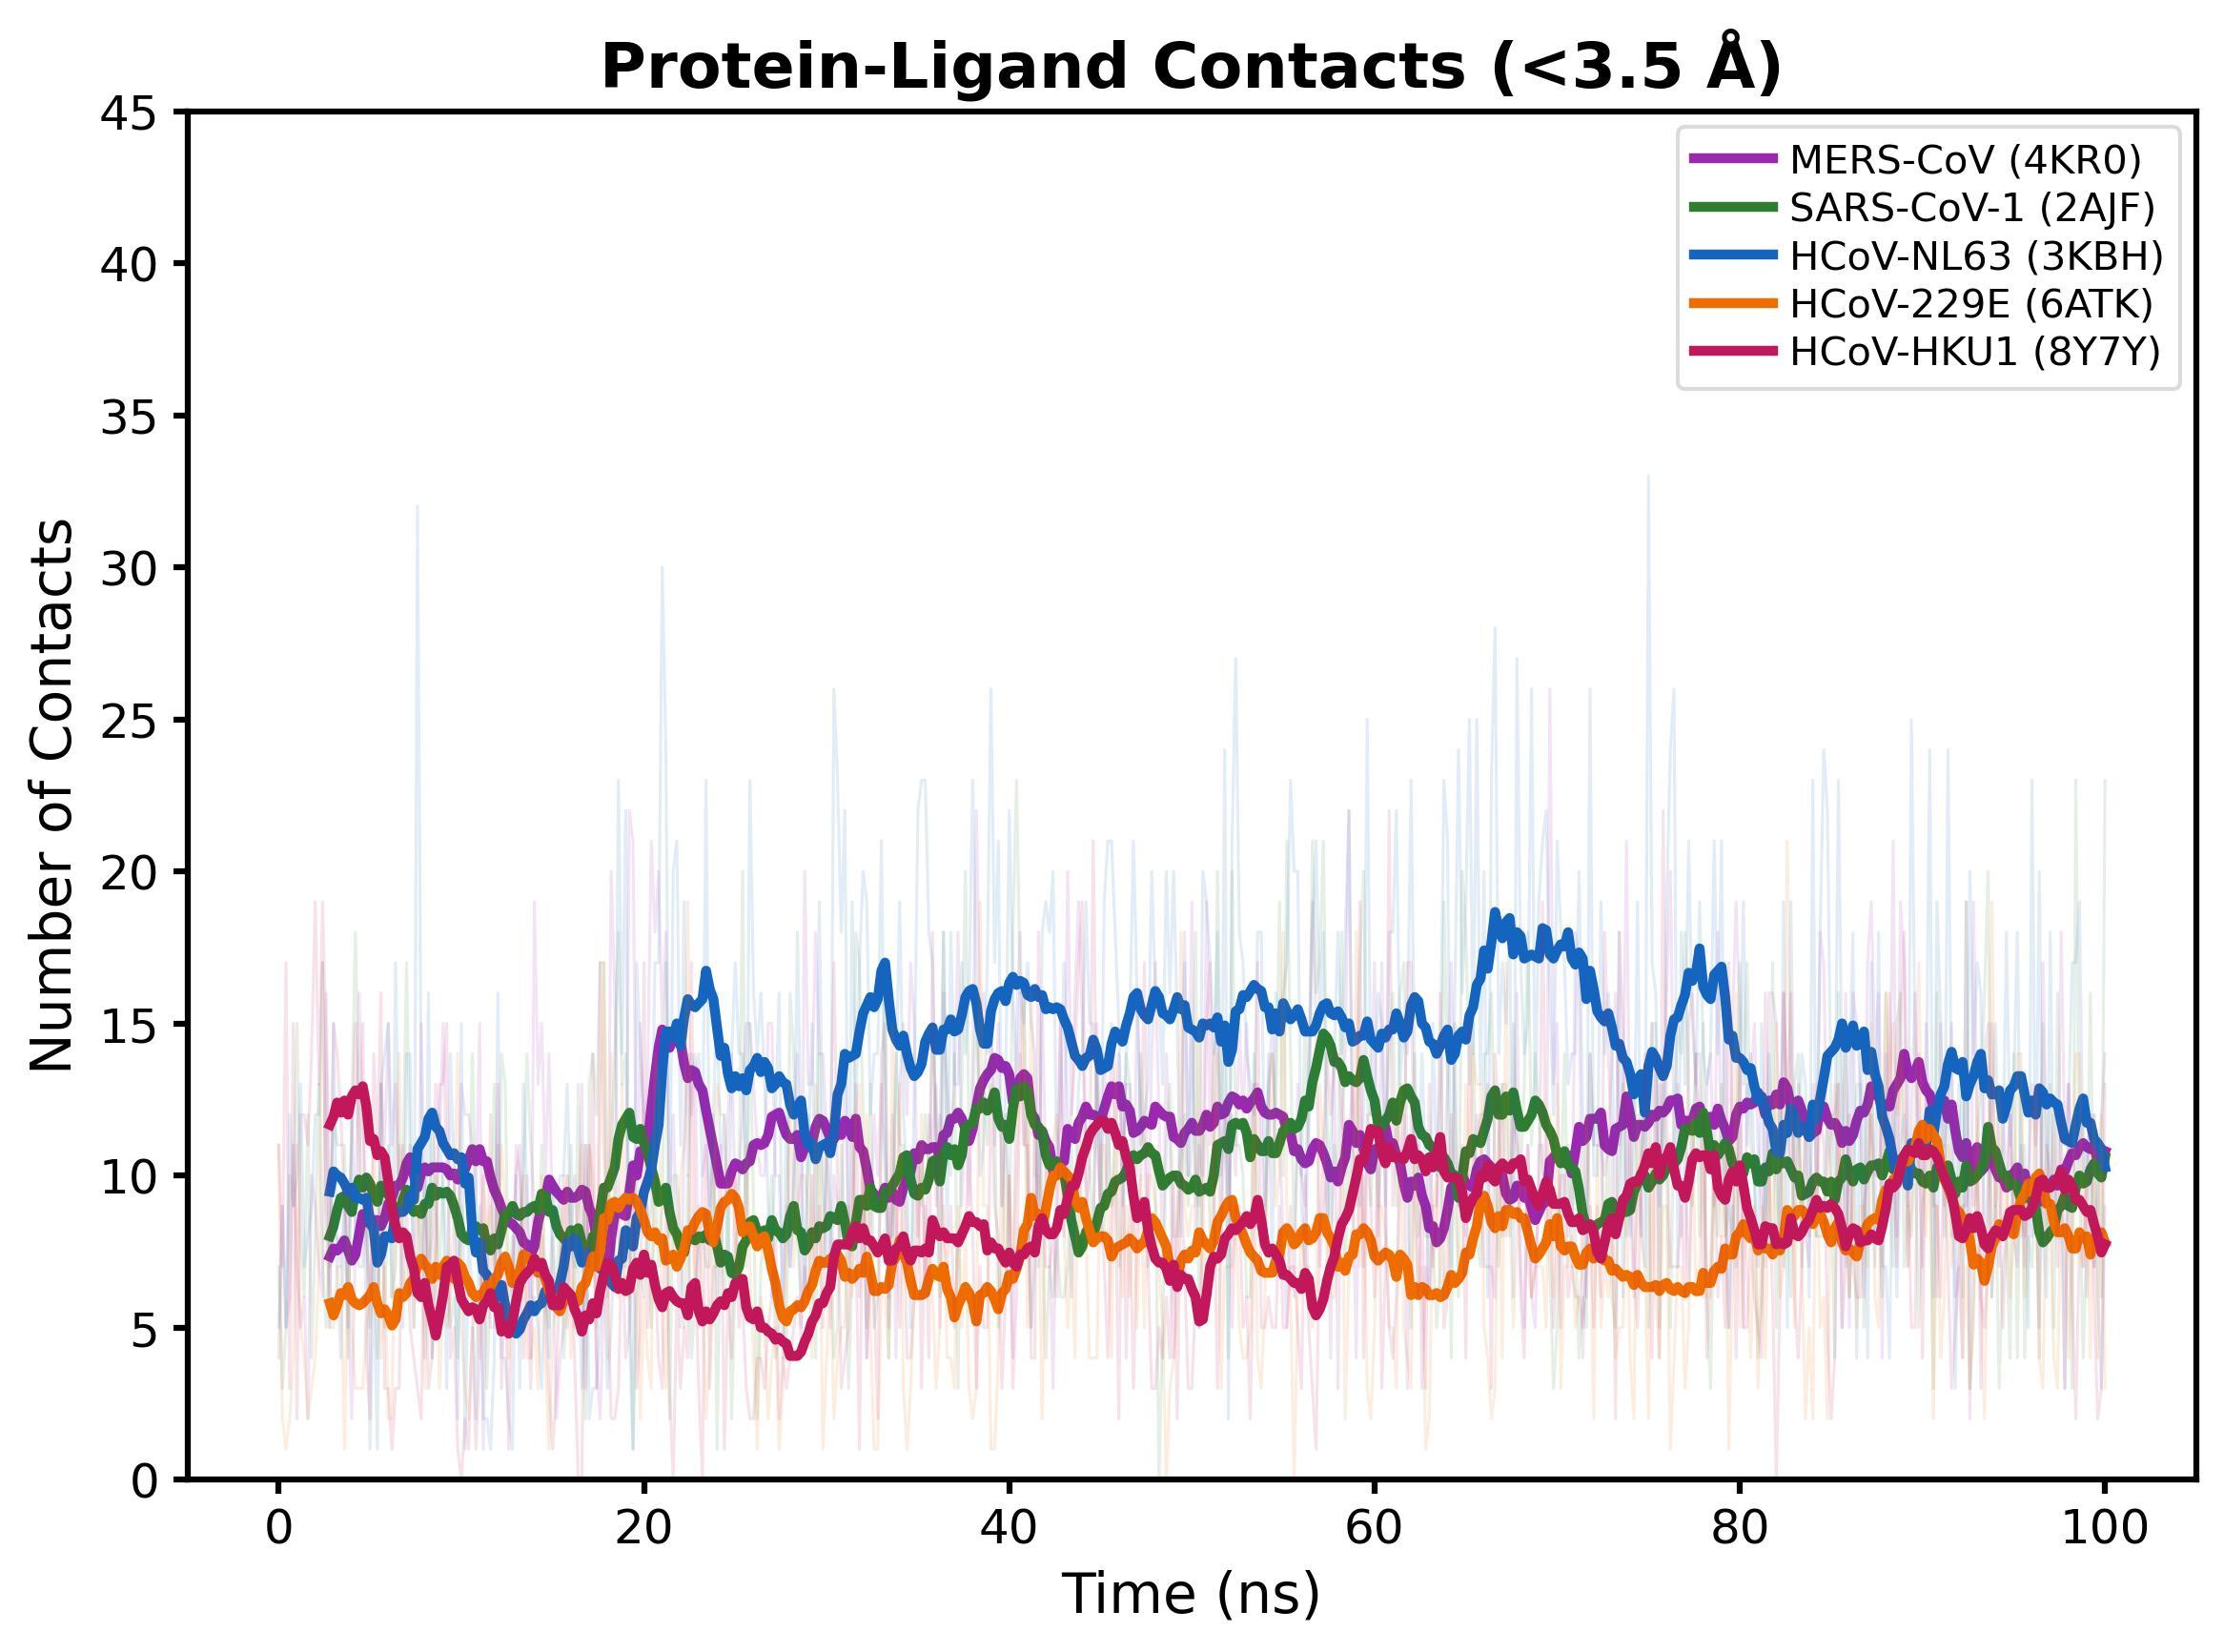
\includegraphics[width=0.75\textwidth]{images/md_contacts.jpg}
\caption{Protein--ligand heavy atom contact counts within 3.5 \AA\ throughout the 100-ns MD trajectories. Faint lines indicate raw contact counts per frame, while solid lines represent the moving average using a 15-frame window, showing persistent close-contact interaction profiles across all five complexes.}
\label{fig:md_contacts}
\end{figure}


\subsection{Per-Residue Flexibility and Global Compactness}
Per-residue C$\alpha$ RMSF profiles (Figure \ref{fig:md_rmsf_rg_stability}A) indicated that peripheral loop regions of the receptor-binding domains displayed elevated flexibility, whereas the receptor-interface regions occupied by CKP-25 generally exhibited comparatively lower fluctuations. This pattern is consistent with local stability of the ligand-bound interface during the production simulations.

\begin{figure}[htbp]
\centering
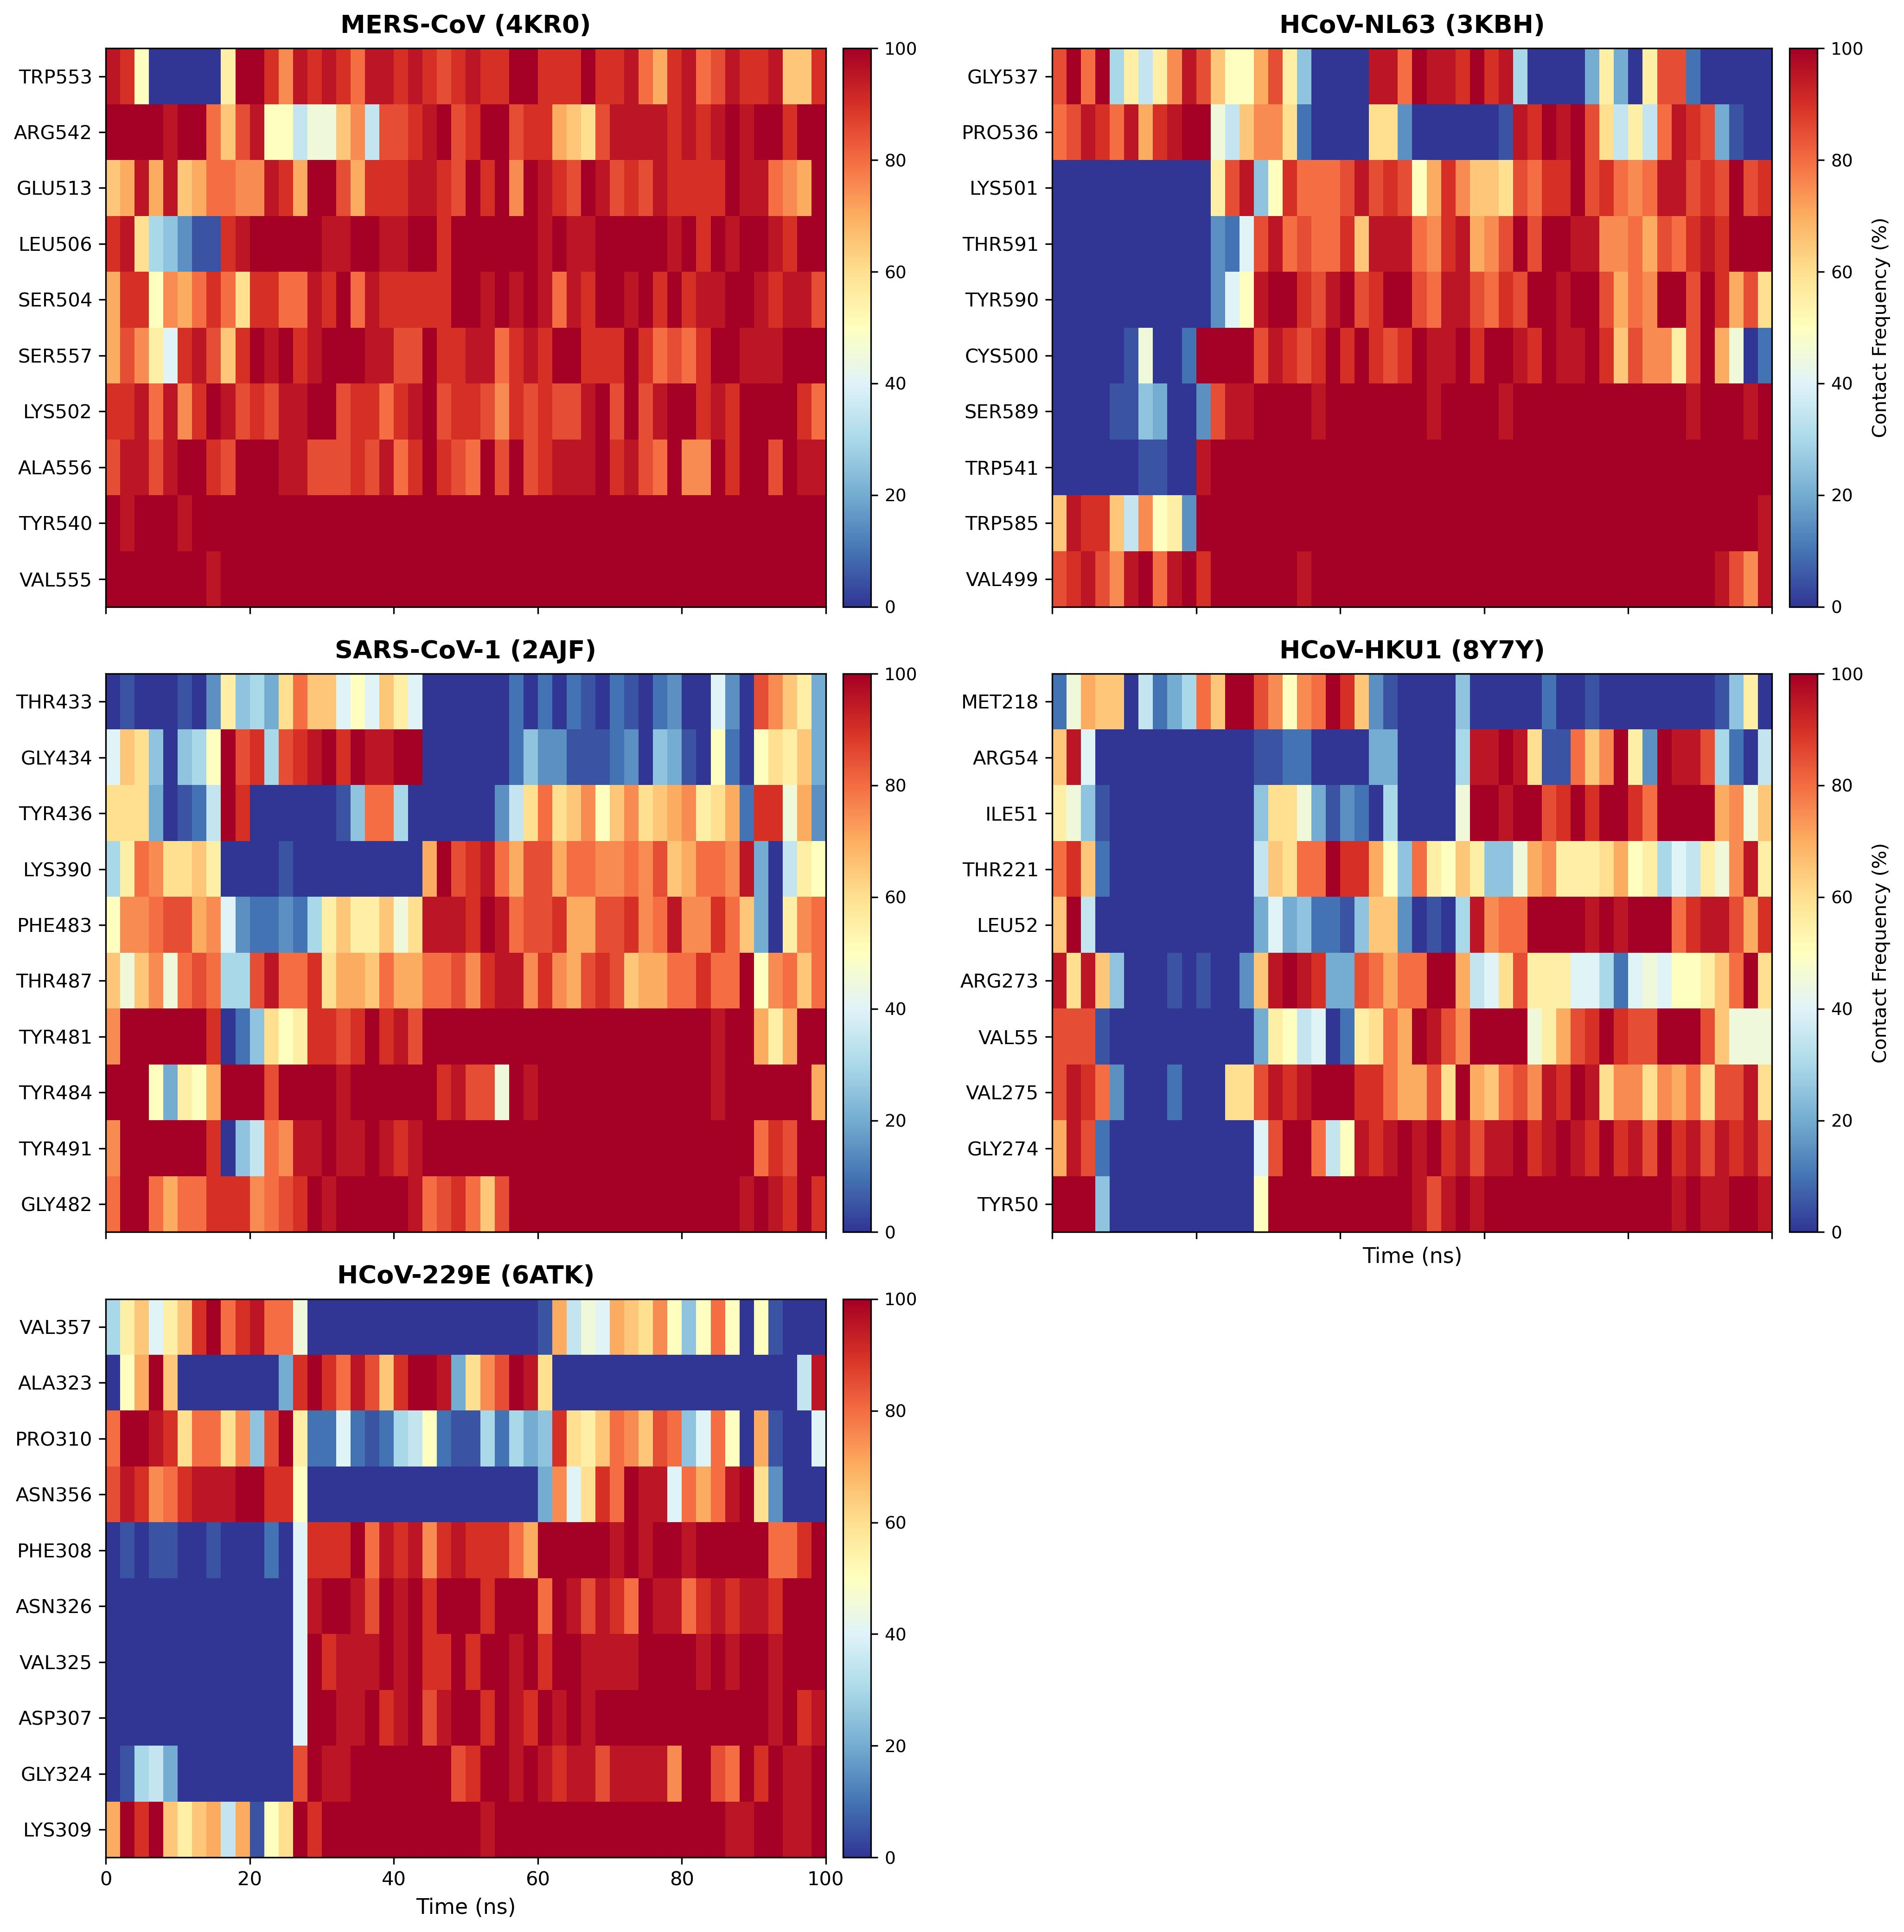
\includegraphics[width=0.95\textwidth]{images/md_contact_heatmap_5panel.jpg}
\caption{\textbf{Residue-specific protein--ligand contact frequency heatmaps} for CKP-25 complexed with the five coronavirus spike targets over the 100-ns MD trajectories. For each target, the top 10 interacting residues are displayed along the y-axis, with contact frequency calculated using a 4.0 Å distance cutoff and binned in 2-ns intervals. The color gradient from blue (low contact frequency) to red (high contact frequency) highlights persistent anchoring of CKP-25 against key aromatic, hydrophobic, and polar interface residues.}
\label{fig:md_contact_heatmap}
\end{figure}


The radius of gyration ($R_g$) was monitored to detect potential large-scale unfolding. The $R_g$ values remained stable with minimal fluctuation across all systems (Figure \ref{fig:md_rmsf_rg_stability}B), supporting the preservation of overall structural compactness throughout the simulations. The mean $R_g$ values over the production trajectories were: MERS-CoV B-spike (18.73 $\pm$ 0.11 \AA), SARS-CoV-1 E-spike (16.99 $\pm$ 0.15 \AA), HCoV-229E E-spike (16.31 $\pm$ 0.10 \AA), HCoV-HKU1 A-spike (19.19 $\pm$ 0.10 \AA), and HCoV-NL63 E-spike (15.37 $\pm$ 0.18 \AA). 

\begin{figure}[htbp]
\centering
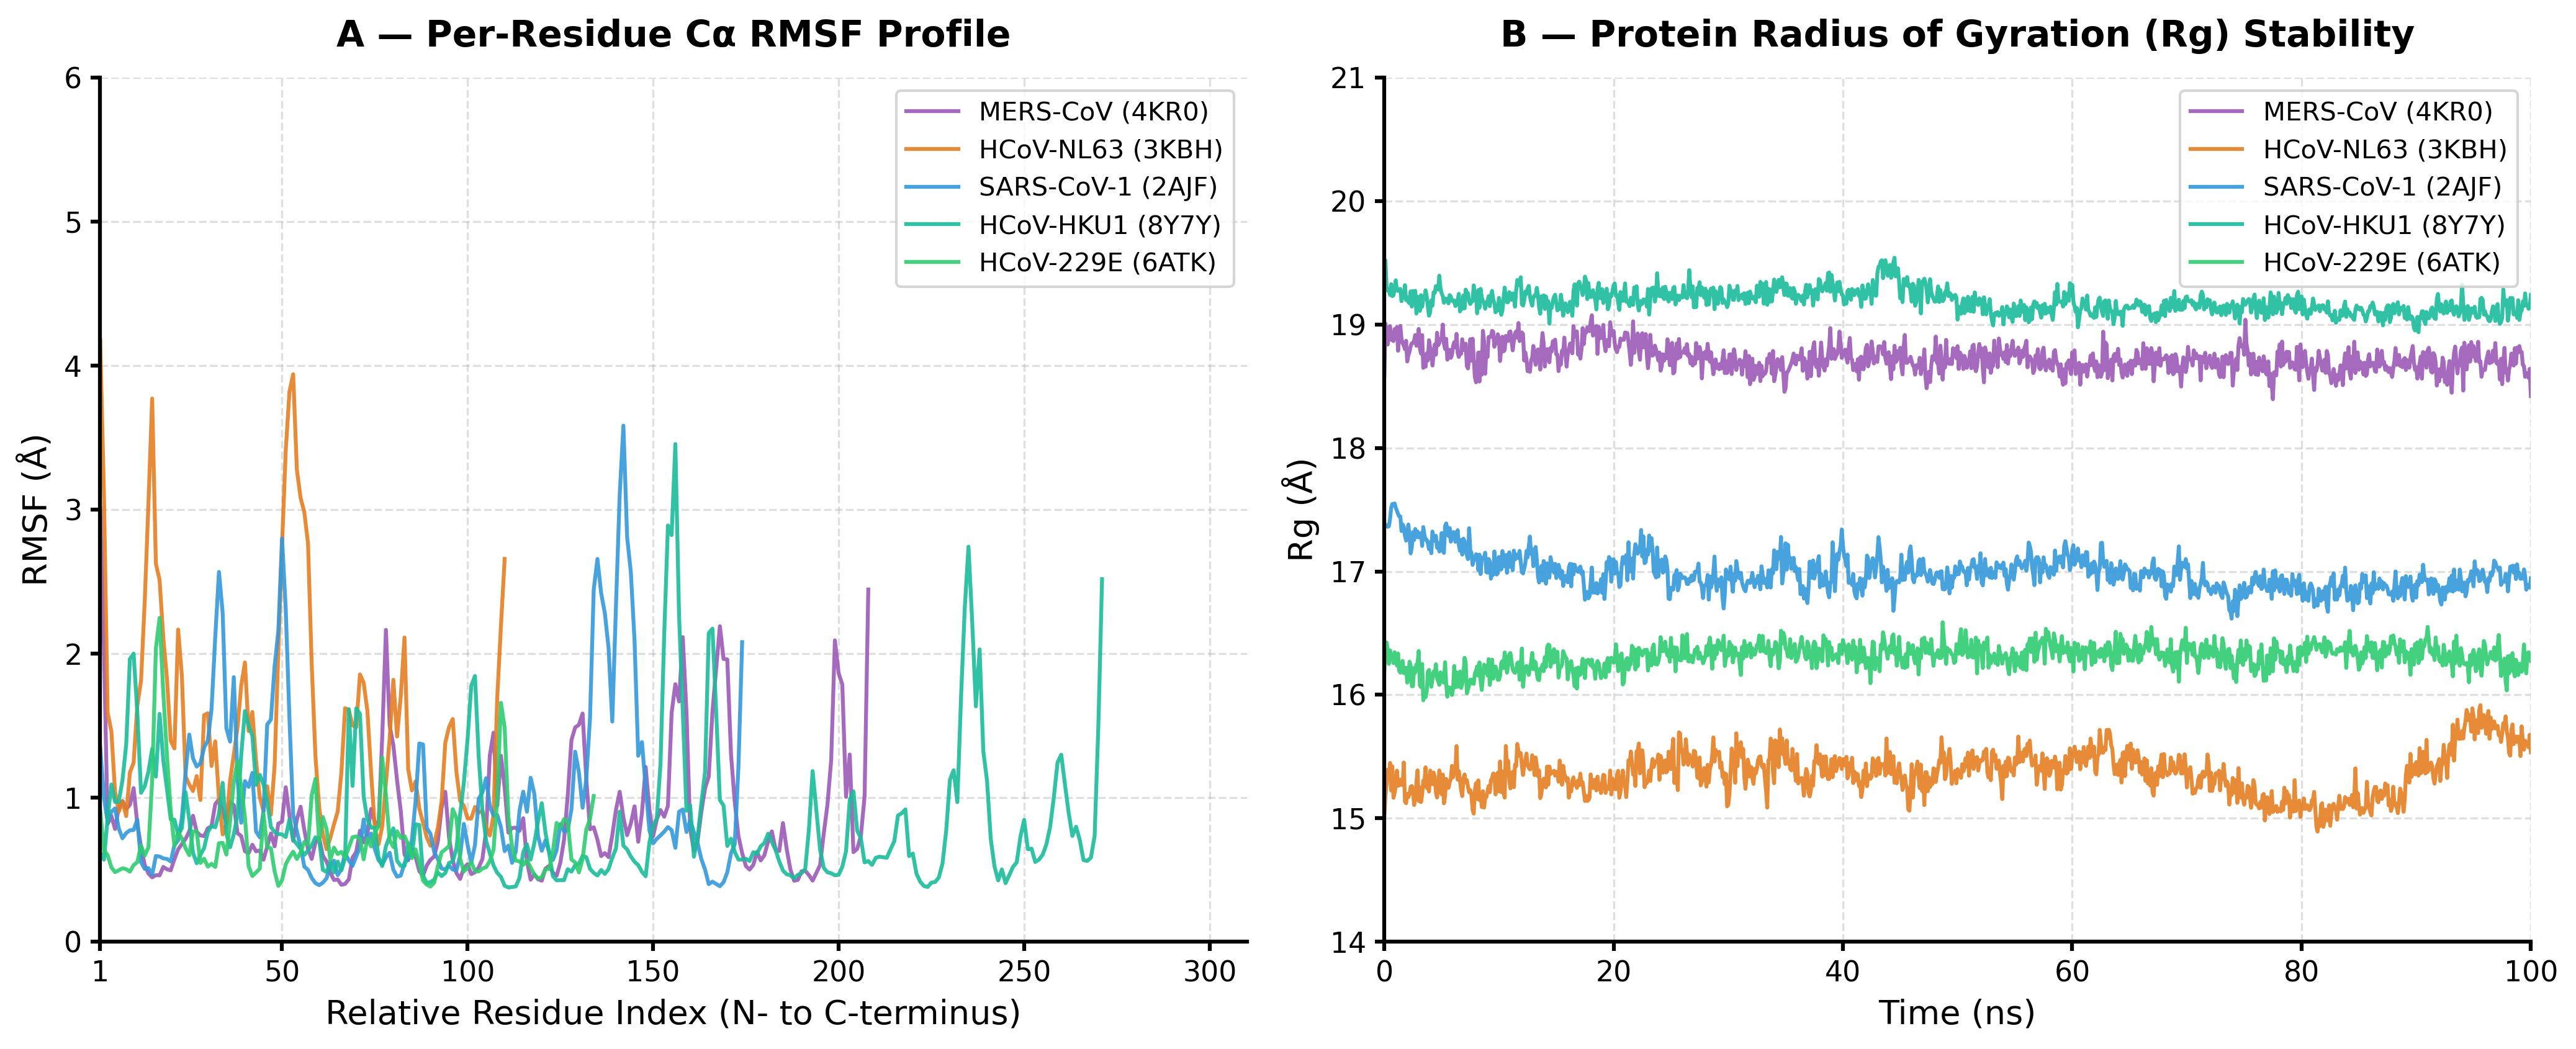
\includegraphics[width=\textwidth]{images/md_rmsf_rg_stability.jpg}
\caption{System dynamics and structural stability analysis for CKP-25 complexed with five human coronavirus spike RBDs. (A) Per-residue C$\alpha$ root-mean-square fluctuation (RMSF) profiles aligned by relative residue index from N- to C-terminus, illustrating elevated flexibility in peripheral loop regions and comparatively lower flexibility around receptor-interface regions. (B) Time-series of the protein radius of gyration ($R_g$) over the 100-ns trajectories, showing stable global compactness across all simulated systems.}
\label{fig:md_rmsf_rg_stability}
\end{figure} 

\subsection{Trajectory Contacts and Polar Interactions}
Total close protein--ligand contacts and polar contacts were analyzed separately to characterize the interaction profile of CKP-25 across the five coronavirus spike targets. Close heavy-atom contacts within 3.5~\AA{} were tracked continuously throughout the trajectories (Figure~\ref{fig:md_contacts}), while residue-level contact frequencies were mapped using a 4.0~\AA{} cutoff (Figure~\ref{fig:md_contact_heatmap}). The HCoV-NL63 complex maintained the highest interaction density, with a mean of $13.57 \pm 5.68$ contacts per frame, closely followed by MERS-CoV ($10.91 \pm 4.20$) and SARS-CoV-1 ($10.25 \pm 4.05$). HCoV-HKU1 ($8.15 \pm 4.24$) and HCoV-229E ($7.32 \pm 3.49$) exhibited slightly lower but highly persistent contact counts.

\begin{figure}[htbp]
\centering
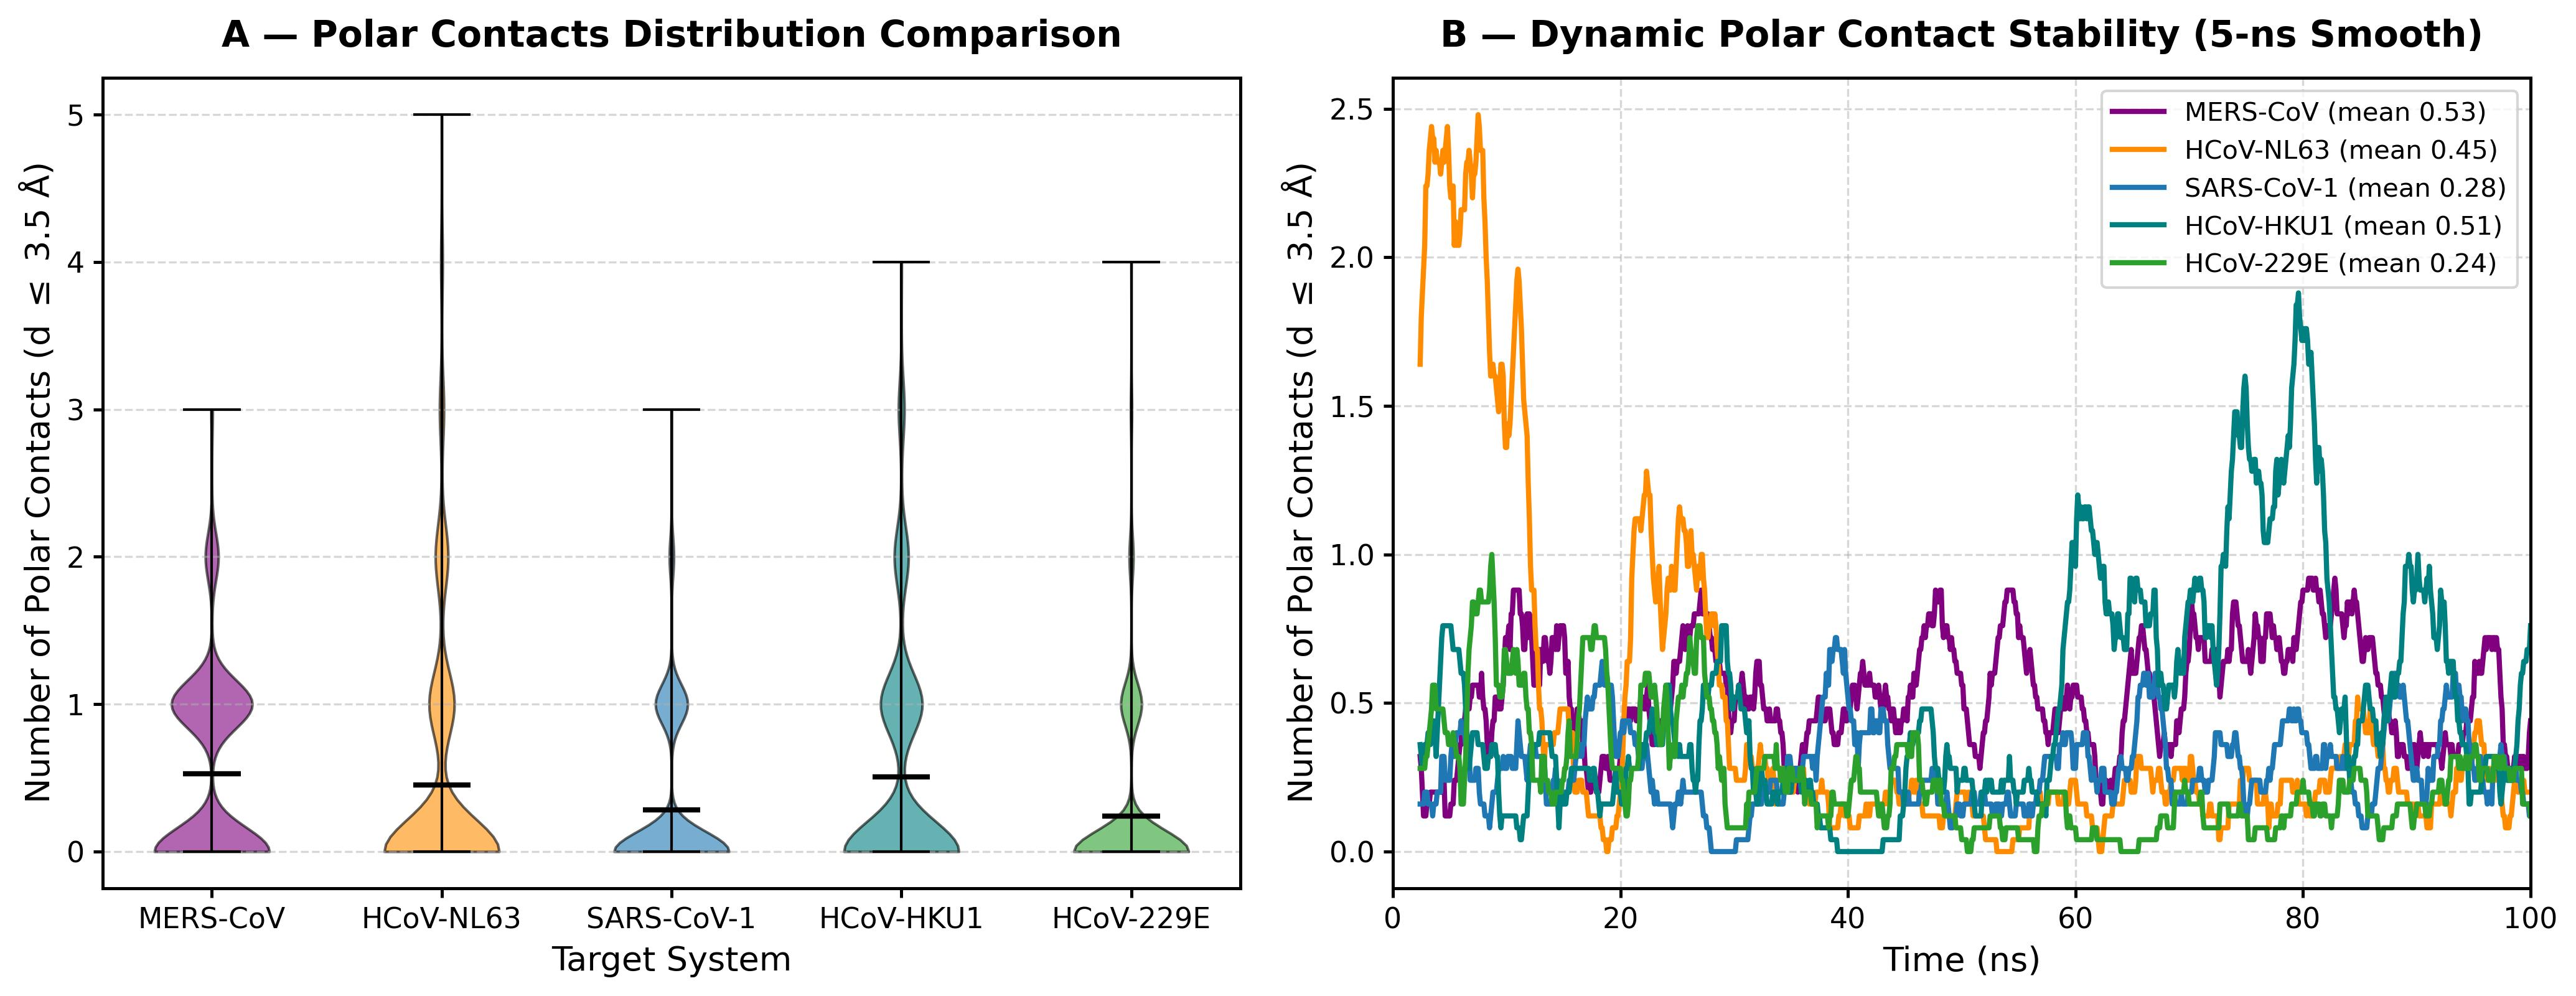
\includegraphics[width=\textwidth]{images/md_polar_contacts_stability.jpg}
\caption{Analysis of protein--ligand polar contacts ($d \leq 3.5$~\AA) for CKP-25 bound to five coronavirus spike receptor-binding domains. (A) Distribution profiles of polar contacts across the 100-ns trajectories represented as violin plots. The black horizontal bars denote the mean values, illustrating that the polar contacts are dynamic and fluctuate mainly between 0, 1, 2, and 3 contacts per frame because of the open-pocket nature of the binding sites. (B) Five-nanosecond moving-average time series showing that, although these polar interactions are transient, they are intermittently formed throughout the 100-ns simulation window.}
\label{fig:md_polar_contacts_stability}
\end{figure}

A detailed analysis of polar contacts ($d \leq 3.5$ \AA) between the polar atoms of CKP-25 and the target spike proteins revealed a highly dynamic interaction network (Figure \ref{fig:md_polar_contacts_stability}). Because the host-receptor interface on the spike protein represents a solvent-exposed, open binding pocket, the ligand's polar groups undergo continuous micro-conformational rotations. Consequently, strict geometric hydrogen bonds (requiring strict donor-acceptor angles) are rare, while broader polar contacts fluctuate rapidly. This dynamic behavior is reflected in the low but persistent average polar-contact counts, ranging from 0.24 contacts per frame for HCoV-229E to 0.53 contacts per frame for MERS-CoV (Figure \ref{fig:md_polar_contacts_stability}A). The moving averages (Figure \ref{fig:md_polar_contacts_stability}B) indicate that these polar interactions are intermittently formed throughout the 100-ns simulations. Rather than relying on a rigid, static hydrogen-bond network, CKP-25 appears to maintain stability primarily through shape-complementary packing, with transient polar contacts acting as secondary stabilizing interactions.

Residues maintaining contact (heavy atoms $< 4.0$ \AA) for $>50\%$ of the simulation represent the core structural anchors:
\begin{itemize}
    \item \textbf{MERS-CoV (4KR0)}: VAL555 (100\%), TYR540 (100\%), SER557 (92.5\%), ALA556 (91.0\%), SER504 (90.0\%), LYS502 (89.6\%), LEU506 (86.6\%).
    \item \textbf{SARS-CoV-1 (2AJF)}: TYR491 (93.0\%), TYR484 (91.5\%), GLY482 (90.5\%), TYR481 (86.6\%), THR487 (77.1\%).
    \item \textbf{HCoV-NL63 (3KBH)}: VAL499 (96.5\%), TRP585 (91.5\%), TRP541 (80.6\%), SER589 (78.1\%), CYS500 (68.7\%).
    \item \textbf{HCoV-229E (6ATK)}: LYS309 (90.5\%), ASP307 (71.6\%), VAL325 (70.6\%), GLY324 (69.2\%), ASN326 (69.2\%).
    \item \textbf{HCoV-HKU1 (8Y7Y)}: TYR50 (77.6\%), VAL275 (69.7\%), GLY274 (68.7\%), VAL55 (53.7\%).
\end{itemize}
This persistent engagement supports a binding mode dominated by shape-complementary van der Waals interactions against hydrophobic/aromatic interface residues. However, because contact frequency measures only structural proximity rather than interaction quality, a high contact count does not always translate directly to stronger thermodynamic stability. To bridge this structural analysis with thermodynamic binding energetics, we carried out MM-GBSA free energy calculations (Section ~\ref{sec:MM-GBSA} ).

\subsection{Thermodynamic Binding Free Energy (MM-GBSA)}
\label{sec:MM-GBSA}
To investigate the thermodynamic driving forces behind CKP-25's binding across the five coronavirus spike targets, we performed Molecular Mechanics-Generalized Born Surface Area (MM-GBSA) calculations. The total binding free energy ($\Delta G_{\text{bind}}$) was decomposed into individual physical energy terms according to Equation \ref{eq:mmgbsa}:
\begin{linenomath}
\begin{equation}\label{eq:mmgbsa}
    \Delta G_{\text{bind}} = \Delta E_{\text{vdw}} + \Delta E_{\text{el}} + \Delta G_{\text{GB}} + \Delta G_{\text{surf}}
\end{equation}
\end{linenomath}
where $\Delta E_{\text{vdw}}$ is the van der Waals interaction energy, $\Delta E_{\text{el}}$ is the electrostatic interaction energy, $\Delta G_{\text{GB}}$ is the polar solvation free energy (modeled using the Generalized Born model, $igb=2$, with a salt concentration of 0.150 M), and $\Delta G_{\text{surf}}$ is the non-polar solvation cavity term calculated from the solvent-accessible surface area (SASA) using the LCPO algorithm. The calculations were averaged over 100 frames extracted at 500-ps intervals from the stable 50--100~ns production window of the MD trajectories. The resulting energy components and total binding free energies are summarized in Table \ref{DG_table}.

\begin{table}[H]
\caption{MM-GBSA thermodynamic binding free energy components (kcal/mol) for CKP-25 complexed with the five coronavirus spike targets, averaged over 100 frames from the stable 50--100~ns production window.\label{DG_table}}
\centering
\begin{tabular}{lcccccc}
\toprule
\textbf{System (PDB)} & $\Delta E_{\text{vdw}}$ & $\Delta E_{\text{el}}$ & $\Delta G_{\text{GB}}$ & $\Delta G_{\text{surf}}$ & $\Delta G_{\text{bind}}$ & \textbf{SD} \\
\midrule
MERS-CoV (4KR0)   & -41.90 & -3.88 & 12.79  & -4.49 & \textbf{-37.47} & $\pm$ 2.72 \\
HCoV-NL63 (3KBH)  & -39.51 & -5.96 & 14.14  & -3.80 & \textbf{-35.12} & $\pm$ 3.50 \\
SARS-CoV-1 (2AJF) & -29.93 & -3.70 & 11.23  & -2.99 & -25.38          & $\pm$ 3.47 \\
HCoV-HKU1 (8Y7Y)  & -29.01 & -1.09 & 7.88   & -2.88 & -25.11          & $\pm$ 3.60 \\
HCoV-229E (6ATK)  & -26.78 & -4.04 & 10.67  & -2.68 & -22.84          & $\pm$ 3.24 \\
\bottomrule
\end{tabular}
\end{table}

The thermodynamic decomposition reveals that the binding of CKP-25 to all five target interfaces is dominated by non-polar interactions. The sum of the non-polar terms ($\Delta E_{\text{vdw}} + \Delta G_{\text{surf}}$) ranges from $-29.46$~kcal/mol for HCoV-229E to a highly favorable $-46.39$~kcal/mol for MERS-CoV, representing close shape-complementary packing and hydrophobic surface burial at the interface. This component analysis also explains the discrepancy between the contact counts and the free energy calculations: although HCoV-NL63 exhibits a higher mean contact count than MERS-CoV ($13.57 \pm 5.68$ vs $10.91 \pm 4.20$ contacts/frame), MERS-CoV demonstrates a slightly better binding affinity. This is because MERS-CoV achieves more optimized van der Waals packing and hydrophobic burial ($\Delta E_{\text{vdw}} = -41.90$ kcal/mol and $\Delta G_{\text{surf}} = -4.49$ kcal/mol) compared to HCoV-NL63 ($\Delta E_{\text{vdw}} = -39.51$ kcal/mol and $\Delta G_{\text{surf}} = -3.80$ kcal/mol), and benefits from a lower polar desolvation penalty ($\Delta G_{\text{GB}} = 12.79$ vs $14.14$ kcal/mol). Thus, MERS-CoV forms fewer but higher-quality contacts that are energetically superior. 

Conversely, the net polar contribution ($\Delta E_{\text{el}} + \Delta G_{\text{GB}}$) is unfavorable across all targets, contributing positive free energies between $+6.63$~kcal/mol (HCoV-229E) and $+8.91$~kcal/mol (MERS-CoV). This discouraging polar contribution arises because the energetic cost of stripping water molecules from the ligand and pocket polar groups (polar desolvation, $\Delta G_{\text{GB}}$) outweighs the direct electrostatic and hydrogen-bonding interactions formed ($\Delta E_{\text{el}}$) at these solvent-exposed interfaces. These findings provide quantitative, physical evidence that CKP-25 acts as a broad-spectrum anchor primarily through shape-complementary hydrophobic/aromatic packing, while polar contacts serve as secondary, fluctuating stabilizers that must overcome substantial desolvation penalties.

\section{Materials and Methods}

\subsection{Target Selection and Receptor-Binding Hotspot Identification}
\label{sec:target_selection}

Experimentally determined structures of human coronavirus spike receptor-binding regions in complex with their respective host receptors or entry mediators were retrieved from the Protein Data Bank (PDB). Targets were selected to represent phylogenetically diverse alpha- and betacoronaviruses, distinct host-receptor usage, and structurally resolved receptor-recognition interfaces suitable for hotspot mapping. The selected systems were:

\begin{itemize}
    \item \textbf{MERS-CoV B-spike}: receptor-binding domain complexed with human dipeptidyl peptidase 4 (DPP4) at 2.70~\AA{} resolution (PDB ID: 4KR0) \cite{lu2013molecular}.
    
    \item \textbf{SARS-CoV-1 E-spike}: receptor-binding domain complexed with human angiotensin-converting enzyme 2 (ACE2) at 2.90~\AA{} resolution (PDB ID: 2AJF) \cite{li2005structure}.
    
    \item \textbf{HCoV-NL63 E-spike}: receptor-binding domain complexed with human ACE2 at 3.31~\AA{} resolution (PDB ID: 3KBH) \cite{wu2009structure}.
    
    \item \textbf{HCoV-229E E-spike}: receptor-binding domain complexed with human aminopeptidase N (APN) at 3.50~\AA{} resolution (PDB ID: 6ATK) \cite{wong2017crystal}.
    
    \item \textbf{HCoV-HKU1 A-spike}: cryo-electron microscopy structure of the spike receptor-binding region complexed with human transmembrane serine protease 2 (TMPRSS2) at 3.24~\AA{} resolution (PDB ID: 8Y7Y) \cite{wang2024tmprss2}.
\end{itemize}

For each complex, the selected viral spike chain was extracted for subsequent docking and molecular dynamics simulations, while the coordinates of the human host partner were removed. Before removal, the host-partner coordinates were used to define the native receptor-recognition hotspot on the viral spike. The hotspot was defined as the set of spike residues containing at least one heavy atom within 4.0~\AA{} of a host-receptor heavy atom, consistent with a commonly used structural cutoff for identifying non-covalent contacts at protein--protein interfaces \cite{jiang2023sars}. The resulting target-specific hotspot residues were used to determine the center and dimensions of the focused docking grid for CKP-25.

\subsection{Molecular Docking Protocol}
Initial binding poses of CKP-25 against the five target spike RBDs were generated using GNINA 1.3, a state-of-the-art molecular docking framework that integrates conventional empirical scoring functions with a deep learning-based 3D convolutional neural network (CNN) for pose scoring and affinity prediction \cite{mcnutt2025gnina}. GNINA 1.3 was selected because its learned CNN scoring functions are designed to capture shape and chemical complementarity in protein--ligand complexes, supporting its use for evaluating CKP-25 binding at solvent-exposed receptor-recognition interfaces.

To perform targeted docking, a focused 3D bounding box (exhaustiveness = 8) was defined separately for each of the five viral spike targets. The box was centered precisely over the identified host-interaction hotspot residues of the isolated spike RBD, rather than using a single uniform box or a global blind search across the entire glycoprotein. Because the five spike RBDs exhibit highly divergent sequence alignments and interface topologies, the box dimensions were custom-tailored for each target to encompass the coordinates of their respective hotspot residues plus a default buffer of 4.0~\AA\ on all six sides. This resulted in target-specific box dimensions of approximately $20\text{ \AA} \times 20\text{ \AA} \times 20\text{ \AA}$ (centered on the native binding region), allowing the ligand to explore conformations capable of blocking host-receptor association.

Importantly, this localized docking approach does not bias the final results: the grid box is used solely to generate the initial starting coordinates for the docking pose. The subsequent 100-ns explicit-solvent MD simulations are completely unrestrained, allowing the ligand and spike protein to undergo conformational changes, relax, or dissociate. Thus, the thermodynamic stability and contact frequencies reported in this study reflect the unrestrained physical behavior of the complexes, independent of the initial docking box boundaries. Poses for each target were ranked primarily by their CNN pose score (which serves as the primary metric in GNINA for structural correctness), while applying a Vina-predicted binding affinity of $< -5.0$ kcal/mol as a secondary thermodynamic filter. The highest-ranked pose that satisfied this Vina filter was selected and extracted as the starting structure for the subsequent MD simulations.

\subsection{Molecular Dynamics Simulations}
All-atom MD simulations were performed using GROMACS 2025.4 with GPU acceleration \cite{abraham2015gromacs}. All simulations were performed on an NVIDIA RTX 3090 GPU with 24 GB of memory.

\textbf{System preparation.} The protein topology for each spike domain was generated with \texttt{gmx pdb2gmx} using the AMBER99SB-ILDN force field \cite{lindorff2010improved} and the TIP3P explicit water model \cite{jorgensen1983comparison}. AMBER99SB-ILDN was selected because of its improved side-chain torsion parameters, which enhance accuracy for side-chain conformation and packing at protein-protein interfaces \cite{lindorff2010improved, gkekas2024ai}. Ligand topology and partial charges were generated with ACPYPE \cite{sousa2012acpype} (interfacing with AmberTools \cite{case2023ambertools} antechamber; gas-phase AM1-BCC charges; net charge = 0), producing GAFF-compatible parameters. Although AM1-BCC does not account for explicit polarization effects in highly aromatic systems, it is heavily validated to reproduce HF/6-31G* electrostatic potentials, providing a highly reliable and computationally efficient charge distribution for GAFF-compatible small molecules. The protein--ligand complex was assembled and placed in a dodecahedral periodic box with a minimum 1.2 nm solute-to-wall distance (\texttt{gmx editconf}), solvated with TIP3P water (\texttt{gmx solvate}), and neutralized by the addition of Na$^+$ and Cl$^-$ counterions (\texttt{gmx genion}).

\textbf{Energy minimization.} Each solvated, charge-neutralized system was subjected to steepest-descent energy minimization (up to 50,000 steps; convergence criterion: $F_{\text{max}} < 1,000$ kJ mol$^{-1}$ nm$^{-1}$) using Particle Mesh Ewald (PME) electrostatics and a Verlet pair-list cutoff scheme ($r_{\text{coulomb}} = r_{\text{vdw}} = 1.0$ nm).

\textbf{Equilibration.} Two sequential equilibration phases were performed with harmonic position restraints on all protein and ligand heavy atoms:
\begin{enumerate}
    \item \textbf{NVT} (100 ps; 50,000 steps $\times$ 2 fs): temperature maintained at 300 K using the V-rescale thermostat ($\tau_T = 0.1$ ps) applied separately to the protein--ligand complex and solvent/ion groups.
    \item \textbf{NPT} (100 ps; 50,000 steps $\times$ 2 fs): pressure maintained at 1.0 bar using the Parrinello--Rahman barostat ($\tau_P = 2.0$ ps; compressibility = $4.5 \times 10^{-5}$ bar$^{-1}$; isotropic coupling); V-rescale thermostat retained.
\end{enumerate}

\textbf{Production MD.} Unrestrained production simulations were run for 100 ns, corresponding to 50,000,000 steps with a 2 fs timestep, for each of the five protein--ligand complexes under the NPT ensemble. Temperature control was maintained with the V-rescale thermostat at 300 K ($\tau_T = 0.1$ ps). Pressure was controlled at 1.0 bar with the Parrinello--Rahman barostat ($\tau_P = 2.0$ ps; compressibility = $4.5 \times 10^{-5}$ bar$^{-1}$). Long-range electrostatics were treated by PME (Fourier grid spacing 0.12 nm). Van der Waals interactions were truncated at 1.0 nm with analytic long-range dispersion corrections applied to both energy and pressure. All bonds involving hydrogen atoms were constrained using the LINCS algorithm. Coordinates were written every 10 ps to compressed XTC trajectory files. The 100-ns simulation length is consistent with established literature for evaluating local pocket occupancy and ligand stability for viral-entry inhibitors \cite{gkekas2024ai}. The initial 200-ps restrained equilibration, consisting of 100 ps under the NVT ensemble followed by 100 ps under the NPT ensemble, was used to relax the solvent and establish the target temperature and density. The complete 100-ns production trajectories were examined for structural stability, ligand retention, and protein--ligand contact persistence. For the end-state MM-GBSA calculations, the first 50 ns of each production trajectory were treated as a relaxation period, and 100 frames were extracted at 500-ps intervals from the equilibrated 50--100~ns window.


\subsection{Trajectory Analysis and Free Energy Calculations}

Structural analyses were performed on the 100-ns production trajectories. Prior to analysis, each trajectory was re-imaged to remove periodic-boundary artifacts and centered on the protein--ligand solute using \texttt{gmx trjconv}. Protein C$_\alpha$ root-mean-square deviation (RMSD), C$_\alpha$ root-mean-square fluctuation (RMSF), radius of gyration ($R_g$), ligand heavy-atom RMSD, and protein--ligand contacts were computed using MDTraj~\cite{mcgibbon2015mdtraj}. Ligand heavy-atom RMSD was calculated after least-squares fitting of the protein C$_\alpha$ atoms to remove global translational and rotational motion. Close protein--ligand contacts were defined as pairs of heavy atoms within 3.5~\AA. Polar contacts were defined as contacts between ligand and protein polar heavy atoms within 3.5~\AA, whereas residue-specific contact frequencies were calculated using a 4.0~\AA{} heavy-atom cutoff \cite{jiang2023sars}.



\section{Discussion}
The findings of this study highlight the value of combining molecular docking with explicit-solvent molecular dynamics (MD) simulations to evaluate the binding stability of candidate broad-spectrum viral entry inhibitors. While static docking frameworks such as GNINA are useful for rapid pose generation and virtual screening, they cannot fully capture the structural plasticity and relaxation of the target binding interface. This limitation is illustrated by the discrepancy between the initial GNINA-reported docking affinities and the final MD/MM-GBSA binding-energy estimates. GNINA predicted HCoV-HKU1 to have the best docking affinity ($-6.76$ kcal/mol), followed by MERS-CoV ($-6.61$ kcal/mol). However, subsequent 100-ns MD simulations and MM-GBSA thermodynamic profiling revealed a different affinity hierarchy: MERS-CoV and HCoV-NL63 emerged as the most favorable targets ($\Delta G_{\text{bind}} < -35$ kcal/mol), while HCoV-HKU1 was relegated to a lower tier ($\Delta G_{\text{bind}} \approx -25.11$ kcal/mol). Under dynamic conditions, the initial static conformation of HCoV-HKU1 relaxed into a less optimal configuration, whereas MERS-CoV and HCoV-NL63 established dense, highly stable contact networks. This outcome highlights the importance of dynamic simulations as a complementary validation step after molecular docking.

A key structural finding is that CKP-25 achieves stable binding by anchoring within hydrophobic and aromatic receptor-interface environments across diverse coronavirus spike proteins. Contact-frequency profiling identified a persistent reliance on shape-complementary van der Waals packing against aromatic and hydrophobic interface residues, including TYR540 in MERS-CoV, TRP541 and TRP585 in HCoV-NL63, and TYR491 and TYR484 in SARS-CoV-1. Although the exact residues differ among viruses, these interaction patterns suggest that CKP-25 can exploit functionally analogous receptor-interface features across divergent human coronaviruses. Because receptor-recognition interfaces are directly involved in host-cell attachment, small molecules that occupy these regions may provide a strategy for interfering with viral entry. Nevertheless, the extent to which these computationally identified interface anchors are mutationally constrained requires further experimental and evolutionary validation.

This structural anchoring is further characterized by the dynamic behavior of polar contacts. While some small-molecule inhibitors rely on rigid, high-occupancy hydrogen bonds, CKP-25 appears to maintain stable binding primarily through shape-complementary packing, supported by transient polar contacts in solvent-exposed, open interface regions. In these regions, polar groups are subject to solvent competition from surrounding water molecules, which can continually form and break hydrogen bonds with both the ligand and the receptor \cite{ladbury1996effect, bissantz2010medicinal}. Since CKP-25 is predominantly hydrophobic and contains only a small number of polar atoms, the primary driver of its broad-spectrum interaction profile is likely close hydrophobic/aromatic packing. The auxiliary polar contacts fluctuate between 0 and 3 contacts per frame as the ligand adapts to the open interface, meaning they are transient rather than static. Their intermittent re-formation throughout the 100-ns trajectories suggests that they provide secondary electrostatic stabilization without requiring a rigid hydrogen-bond network. This dynamic polar engagement, combined with persistent hydrophobic and aromatic contacts, supports CKP-25’s stable interaction profile across all five coronavirus spike targets.

The thermodynamic data calculated via MM-GBSA stratified the five coronavirus targets into two predicted binding-energy tiers. MERS-CoV and HCoV-NL63 formed the most favorable tier, while SARS-CoV-1, HCoV-HKU1, and HCoV-229E occupied a moderate predicted binding-energy tier. Because the standard deviation for MM-GBSA calculations in these complex systems is approximately $\pm 3.0$ kcal/mol, the minor intra-tier variations, such as the difference between MERS-CoV and HCoV-NL63 should not be over-interpreted. The more robust conclusion is that CKP-25 shows a stronger predicted preference for the MERS-CoV and HCoV-NL63 interfaces than for the remaining three targets. Furthermore, these free-energy values should be interpreted strictly as relative computational estimates rather than absolute experimental binding free energies. Because MM-GBSA does not include rigorous conformational entropic penalties ($-T\Delta S$), the calculated absolute free energies may be over-encouraging; therefore, direct conversion to experimental dissociation constants (Kd) would be inappropriate.

While this study provides computational evidence supporting CKP-25’s broad-spectrum potential, several limitations must be acknowledged. First, the 100-ns simulation window supports local pocket stability but cannot fully capture larger-scale conformational changes associated with spike protein activation or viral membrane fusion. Second, the simulations were performed on isolated spike receptor-binding regions in explicit water, omitting the lipid envelope, full spike-trimer context, and the extensive glycan shield that covers the spike protein in vivo. Although receptor-binding interfaces must remain at least partially accessible to allow host interaction, surrounding glycans and higher-order spike architecture could influence ligand access and binding stability. Consequently, future work should evaluate CKP-25 in the context of fully glycosylated spike trimers and validate these computational predictions through in vitro assays, such as surface plasmon resonance (SPR) or biolayer interferometry binding studies, as well as pseudotyped-virus entry or neutralization assays.

\section{Conclusions}
By combining targeted deep-learning-guided molecular docking with all-atom explicit-solvent molecular dynamics simulations, we computationally show that CKP-25 maintains stable predicted binding across a phylogenetically diverse panel of five coronavirus spike glycoproteins. Our dynamic evaluations reveal a stratified thermodynamic preference, identifying MERS-CoV and HCoV-NL63 as the best predicted binding targets. These findings highlight the importance of dynamic simulations as a complementary validation step after static docking and support CKP-25 as a promising broad-spectrum receptor-interface binding scaffold for future experimental evaluation as a viral entry inhibitor.

%%%%%%%%%%%%%%%%%%%%%%%%%%%%%%%%%%%%%%%%%%
\vspace{6pt} 

\supplementary{The following supporting information can be downloaded at: \url{www.mdpi.com/xxx/s1}}

% \authorcontributions{Conceptualization, Anonymous; methodology, Anonymous; software, Anonymous; validation, Anonymous; formal analysis, Anonymous; investigation, Anonymous; resources, Anonymous; data curation, Anonymous; writing---original draft preparation, Anonymous; writing---review and editing, Anonymous; visualization, Anonymous; supervision, Anonymous; project administration, Anonymous. The author has read and agreed to the published version of the manuscript.}
\authorcontributions{Conceptualization, S.P.; methodology, A.-M.P. and S.P.; software, A.-M.P.; validation, A.-M.P.; formal analysis, A.-M.P.; investigation, A.-M.P.; data curation, A.-M.P.; writing---original draft preparation, A.-M.P.; writing---review and editing, A.-M.P. and S.P.; visualization, A.-M.P.; supervision, F.A. and P.D. All authors have read and agreed to the published version of the manuscript.}



\funding{This research received no external funding.}

\institutionalreview{Not applicable.}

\informedconsent{Not applicable.}

\dataavailability{The data presented in this study are available on request from the corresponding author.} 

\acknowledgments{We thank our collaborators and partners for their valuable advice and support.}

\conflictsofinterest{The authors declare no conflicts of interest.} 

\abbreviations{Abbreviations}{
The following abbreviations are used in this manuscript:
\\
\noindent 
\begin{tabular}{@{}ll}
HCoV & Human Coronavirus \\
SARS & Severe Acute Respiratory Syndrome \\
MERS & Middle East Respiratory Syndrome \\
RBD & Receptor-Binding Domain \\
MD & Molecular Dynamics \\
MM-GBSA & Molecular Mechanics-Generalized Born Surface Area \\
RMSD & Root-Mean-Square Deviation \\
RMSF & Root-Mean-Square Fluctuation \\
Rg & Radius of Gyration \\
SASA & Solvent-Accessible Surface Area \\
PDB & Protein Data Bank \\
CNN & Convolutional Neural Network \\
PME & Particle Mesh Ewald \\
LINCS & Linear Constraint Solver \\
GAFF & General Amber Force Field
\end{tabular}
}

%%%%%%%%%%%%%%%%%%%%%%%%%%%%%%%%%%%%%%%%%%
\begin{adjustwidth}{-\extralength}{0cm}
\reftitle{References}
\bibliography{refs}

\PublishersNote{}
\end{adjustwidth}
\end{document}
